\subsection{群作逆紧作用的性质}

命题 3. 若拓扑群 G 逆紧作用于拓扑空间 X，则轨道空间 X/G 是豪斯多夫的。若 G 还是豪斯多夫的，则 X 也是豪斯多夫的。

设 \(C \subset X \times X\) 是等价关系 \(R\)（由 \(G\) 定义在 \(X\) 上的）的图；则 \(C\) 是 \(G \times X\) 在映射 \(\theta : (s, x) \to (x, s.x)\) 下的像。由于 \(\theta\) 是逆紧的，\(C\) 在 \(X \times X\) 中闭（第一章，§ 10，第 1 节，命题 1）。由于关系 \(R\) 是开的（§ 2，第 4 节，引理 2），由此推出 \(X/G\) 是豪斯多夫的（第一章，§ 8，第 3 节，命题 8）。

现在设 G 是豪斯多夫的。则映射 \(x \to (e, x)\)（X 到 \(G \times X\) 中的映射）是 X 到 \(G \times X\) 的一个闭子空间上的同胚，因而是逆紧的（第一章，§ 10，第 1 节，命题 2）。把这个映射与映射 \((s, x) \to (x, s.x)\)（\(G \times X\) 到 \(X \times X\) 中的映射，由假设它是逆紧的）复合，就得到 X 到 \(X \times X\) 中的一个逆紧映射，即对角映射 \(x \to (x, x)\)。于是对角线 \(\Delta\)（\(X \times X\) 的对角线）在 X 中是闭的，因此 X 是豪斯多夫的。

命题 4. 设 G 是逆紧作用于拓扑空间 X 的一个拓扑群，并设 x 是 X 的一点。用 G.x 表示 x 的轨道，用 \(K_{x}\) 表示 x 的稳定子群。那么：

\begin{enumerate}
\def\labelenumi{\alph{enumi})}
\item
  映射 \(s \to s.x\) 是 \(G\) 到 \(X\) 中的逆紧映射。
\item
  \(\mathbf{K}_x\) 是拟紧的。
\item
  \(\mathbf{G} / \mathbf{K}_x\) 到 \(\mathbf{G}.x\) 上的典范映射是同胚。
\item
  轨道 G.x 在 X 中是闭的。
\end{enumerate}

\(\{x\} \times X\) 在 \(\theta : (s, x) \to (x, s.x)\) 下的逆像是 \(G \times \{x\}\)；因此，由第一章 § 10 第 1 节命题 3，\(\theta\) 在 \(G \times \{x\}\) 上的限制是 \(G \times \{x\}\) 到 \(\{x\} \times X\) 中的逆紧映射，由此得 a)。由于 \(K_x\) 是 \(x\) 在 \(s \to s.x\) 下的逆像，故 b) 由第一章 § 10 第 2 节定理 1 得出。c) 与 d) 是 a) 的推论，这依据第一章 § 10 第 1 节命题 2 与命题 5 b)。

注. 命题 4 表明，若拓扑群 G 逆紧作用于齐性空间 G/H，则子群 H 是拟紧的（从而当 G 是豪斯多夫的时它是紧的）。可以证明，这也是 G 逆紧作用于 G/H 的一个充分条件（习题 3）。

命题 5. 设 G（相应地，G'）是连续作用于拓扑空间 X（相应地，X'）的拓扑群。设 φ 是 G 到 \(\mathbf{G}'\) 中的一个连续同态，并设 \(\psi\) 是 X 到 \(\mathbf{X}'\) 中与 \(\varphi\) 相容的连续映射（ \(\S 2\) ，第 4 节）。那么：

\begin{enumerate}
\def\labelenumi{(\roman{enumi})}
\item
  若 \(\varphi\) 是满射，\(\psi\) 是满射且逆紧的，并且 \(\mathbf{G}\) 逆紧作用于 \(\mathbf{X}\)，则 \(\mathbf{G}'\) 逆紧作用于 \(\mathbf{X}'\)。
\item
  若 \(\varphi\) 是逆紧的，\(\mathbf{G}'\) 逆紧作用于 \(\mathbf{X}'\)，且 \(\mathbf{X}\) 是豪斯多夫的，则 \(\mathbf{G}\) 逆紧作用于 \(\mathbf{X}\)。
\end{enumerate}

为证 (i)，考虑交换图

\[
\begin{array}{c c c c} \mathbf {G} & \times \mathbf {X} \xrightarrow {\theta} \mathbf {X} & \times \mathbf {X} \\ \alpha & \downarrow & & \downarrow \beta \\ \mathbf {G} ^ {\prime} & \times \mathbf {X} ^ {\prime} \xrightarrow {\theta^ {\prime}} \mathbf {X} ^ {\prime} & \times \mathbf {X} ^ {\prime} \end{array}
\]

其中 \(\alpha = \varphi \times \psi\)，\(\beta = \psi \times \psi\)。由假设，\(\theta\) 是逆紧的；\(\beta\) 也是逆紧的{[}第一章，§ 10，第 1 节，命题 4a){]}；于是 \(\beta \circ \theta = \theta' \circ \alpha\) 是逆紧的{[}第一章，§ 10，第 1 节，命题 5a){]}。由于 \(\alpha\) 是满射，由此推出 \(\theta'\) 是逆紧的{[}第一章，§ 10，第 1 节，命题 5b){]}。

为证 (ii)，考虑超滤子 \(\mathfrak{U}\)，它定义在 \(\mathbf{G} \times \mathbf{X}\) 上，使得映射

\[
(s, x) \rightarrow s. x \quad \text { and } \quad (s, x) \rightarrow x
\]

关于 \(\mathfrak{U}\) 分别收敛于 \(y_0\) 与 \(x_0\)。由此推出 \((s, x) \to \varphi(s). \psi(x)\) 与 \((s, x) \to \psi(x)\) 关于 \(\mathfrak{U}\) 收敛。由于 \(\mathbf{G}'\) 逆紧作用于 \(\mathbf{X}'\)，这就意味着（第 1 节）\((s, x) \to \varphi(s)\) 关于 \(\mathfrak{U}\) 收敛于一点 \(s_0' \in \mathbf{G}'\)。由于 \(\varphi\) 是逆紧的，我们推出（第一章，§ 10，第 2 节，定理 1）\((s, x) \to s\) 关于 \(\mathfrak{U}\) 收敛于一点 \(s_0 \in \mathbf{G}\)。于是在 \(\mathbf{X}\) 中极限的唯一性表明 \(y_0 = s_0 x_0\)，从而 \(\mathbf{G}\) 逆紧作用于 \(\mathbf{X}\)（第 1 节）。

\subsection{在拓扑空间上自由作用的群}

定义 2. 设 G 是作用于一个集合 X 上的群。如果 X 的每个元素的稳定子群都是 \(\{e\}\)，换句话说，如果关系 \(s.x = x, s \in G, x \in X\) 蕴含 s = e，则称 G 自由作用于 X。

例. 设 G 是群，H 是 G 的子群。则 H 通过（左或右）平移自由作用于 G。

设 G 是自由作用于集合 X 的群，R 是 G 在 X 上定义的等价关系，\(C \subset X \times X\) 是 R 的图。若 \((x, y) \in C\)，则存在 \(s \in G\) 使得 s.x = y；且 s 是唯一的，因为 \(s.x = s'.x\) 蕴含 \(s'^{-1}s.x = x\)，从而 \(s'^{-1}s = e\)（由于 G 自由作用）。让 \((x, y) \in C\) 对应于使 s.x = y 的唯一的 \(s \in G\)，我们就定义了一个映射 \(\varphi: C \to G\)，我们称它为 C 到 G 中的典范映射。采用此记号：

命题 6. 设 G 是连续作用于拓扑空间 X 的拓扑群，且设 G 自由作用于 X。则 G 逆紧作用于 X 当且仅当下述条件成立：

(FP) 由 G 所定义的等价关系的图 C 在 \(X \times X\) 中闭，且典范映射 \(\varphi: C \rightarrow G\) 连续。

集合 C 是映射 \(\theta: (s, x) \to (x, s.x)\)（\(\mathbf{G} \times \mathbf{X}\) 到 \(\mathbf{X} \times \mathbf{X}\) 中的映射）的像。我们知道（第一章，§ 10，第 1 节，命题 2），\(\theta\) 是逆紧的当且仅当 C 在 \(\mathbf{X} \times \mathbf{X}\) 中闭，并且（若用 \(\theta'\) 表示把 \(\theta\) 看作 \(\mathbf{G} \times \mathbf{X}\) 到 C 中的映射）\(\theta'\) 是同胚。现在，假设蕴含 \(\theta'\) 是双射且其逆是映射 \((x, y) \to (\varphi(x, y), x)\)。于是 \(\theta'\) 是同胚当且仅当 \(\varphi\) 连续。

\subsection{作逆紧作用的局部紧群}

命题 7. 设 G 是连续作用于豪斯多夫空间 X 的局部紧群。则 G 逆紧作用于 X 当且仅当：对 X 的每一对点 x, y，存在 x 的邻域 \(V_{x}\) 与 y 的邻域 \(V_{y}\)，使得集合 K——由 \(s \in G\) 中满足 \(s \cdot V_{x} \cap V_{y} \neq \emptyset\) 的所有 s 组成——在 G 中相对紧。

设 F 是把无穷远点 \(\omega\) 添加到 G 上所得的紧空间，并设 \(\Gamma\) 是 \(\rho: (s, x) \to s.x\) 的图，把它看作 \(F \times X \times X\) 的一个子集。我们来证明，如果 \(pr_{23}\) 在 \(\Gamma\) 上的限制是逆紧的，那么 \(\Gamma\) 在 \(F \times X \times X\) 中是闭的。事实上，这一假设蕴含映射 \(u: (t, s, x, y) \to (t, x, y)\)（\(F \times \Gamma\) 到 \(F \times X \times X\) 中的映射）是闭映射。若 \(\Gamma'\) 是由点 \((s, s)\) 组成的集合，这些点位于 \(F \times G\) 中且 \(s \in G\)，则 \(\Gamma'\) 在 \(F \times G\) 中闭，因为它是典范单射 \(G \to F\) 的图（第一章，§8，第 1 节，命题 2 的推论 2）；于是交 \((\Gamma' \times X \times X) \cap (F \times \Gamma)\) 在 \(F \times \Gamma\) 中闭，并且立即可以看出它在 u 下的像正是把 \(\Gamma\) 看作 \(F \times X \times X\) 的子集时的那个集合；从而 \(\Gamma\) 在 \(F \times X \times X\) 中闭。另一方面，我们有 \((\{\omega\} \times X \times X) \cap \Gamma = \emptyset\)。于是由 F 的定义，对每一点 \((x, y) \in X \times X\)，存在 \((x, y)\) 在 \(X \times X\) 中的一个邻域 W 和 G 的一个紧子集 K，使得

\[
((\mathbf {G} - \mathbf {K}) \times \mathbf {W}) \cap \Gamma ;
\]

为空；由于可取 W 为形如 \(V_{x} \times V_{y}\) 的邻域，其中 \(V_{x}\) 与 \(V_{y}\) 分别是 X 中 x 与 y 的邻域，断言“((G - K) × W) ∩ Γ = ∅”就成为“若 s∉K，则 s.Vx∩Vy=∅”。这样我们就证明了命题所述条件的必要性。反之，设此条件成立；设 A 是由超滤子 \(\mathfrak{F}\) 滤化的集合，并设 \(\alpha \to (s_{\alpha}, x_{\alpha})\) 是 A 到 \(G \times X\) 中的映射，使得 \(\lim_{\mathfrak{F}} x_{\alpha} = x\) 且 \(\lim_{\mathfrak{F}} s_{\alpha}\cdot x_{\alpha} = y\)。设 K、Vx 与 Vy 满足命题的条件。由假设，存在集合 \(M \in \mathfrak{F}\)，使得若 \(\alpha \in M\)，则 \(x_{\alpha} \in V_{x}\) 且 \(s_{\alpha}\cdot x_{\alpha} \in V_{y}\)，从而 \(s_{\alpha} \in K\)。这表明 \(\alpha \to s_{\alpha}\) 关于 \(\mathfrak{F}\) 收敛，证毕。

若 G 是紧的，命题 7 的条件平凡地成立；这样我们重新得到命题 2a)。

命题 7 特别表明，连续作用于豪斯多夫空间 X 的离散群 G 逆紧作用于 X 当且仅当：对 X 的每一对点 \((x, y)\)，存在 x 的邻域 \(V_{x}\) 与 y 的邻域 \(V_{y}\)，使得由 \(s \in G\) 中满足 \(s \cdot V_{x} \cap V_{y} \neq \emptyset\) 的点组成的集合是有限的。

命题 8. 设 G 是逆紧作用于豪斯多夫空间 X 的离散群。设 x 是 X 的一点，\(K_{x}\) 是 x 的稳定子群。那么：

\begin{enumerate}
\def\labelenumi{\alph{enumi})}
\item
  子群 \(K_{x}\) 是有限的，并且存在 \(U \subset X\) 的开集，它包含 x，在 \(K_{x}\) 下稳定，并且在它上面由 G 所定义的关系诱导的等价关系就是由 \(K_{x}\) 定义的等价关系。
\item
  典范映射 \(\mathbf{U} / \mathbf{K}_x\to \mathbf{X} / \mathbf{G}\) 是 \(\mathbf{U} / \mathbf{K}_x\) 到 \(x\) 的类在 \(\mathbf{X} / \mathbf{G}\) 中的一个开邻域上的同胚。
\end{enumerate}

由命题 7，\(\mathbf{K}_x\) 是有限的。为构造满足所需条件的开集 \(\mathbf{U}\)，首先注意，由命题 7 存在开集 \(\mathrm{U}_0\)（包含 \(x\)），使得集合 \(\mathbf{K}\)——由 \(s \in \mathbf{G}\) 中满足 \(s. \mathrm{U}_0 \cap \mathrm{U}_0 \neq \emptyset\) 的那些 s 组成——是有限的。显然 \(\mathbf{K}_x \subset \mathbf{K}\)；设 \(s_1, \ldots, s_n\) 是 \(\mathbf{K} - \mathbf{K}_x\) 的元素。若令 \(x_i = s_i.x\)（ \(1 \leqslant i \leqslant n\)），则 \(x_i \neq x\) 对每个 \(i\) 成立；由于 \(\mathbf{X}\) 是豪斯多夫的，对每个指标 \(i\) 存在开邻域 \(\mathrm{V}_i\)（包含 \(x\)）与开邻域 \(\mathrm{V}_i'\)（包含 \(s_i.x\)），使得 \(\mathrm{V}_i \cap \mathrm{V}_i' = \emptyset\)。令 \(\mathrm{U}_i = \mathrm{V}_i \cap s_i^{-1}. \mathrm{V}_i'\)；则 \(\mathrm{U}_i\) 显然是开的且包含 \(x\)，并且我们有 \(\mathrm{U}_i \cap s_i. \mathrm{U}_i \subset \mathrm{V}_i \cap \mathrm{V}_i' = \emptyset\)。令 \(\mathrm{U}' = \mathrm{U}_0 \cap \mathrm{U}_1 \cap \ldots \cap \mathrm{U}_n\)；\(\mathrm{U}'\) 是开的，包含 \(x\)，并且 \(\mathrm{U}' \cap s. \mathrm{U}' = \emptyset\) 对 \(s \notin \mathbf{K}_x\) 成立。令 \(\mathrm{U} = \bigcap_{t \in \mathbf{K}_x} t. \mathrm{U}'\)，我们最终得到一个开集，它在 \(\mathbf{K}_x\) 下稳定，包含 \(x\)，并且 \(\mathrm{U} \cap s. \mathrm{U} = \emptyset\) 对 \(s \notin \mathbf{K}_x\) 成立：\(\mathrm{U}\) 就是所要求的开集。

典范映射 \(\mathbf{U} / \mathbf{K}_x\to \mathbf{X} / \mathbf{G}\) 是 \(\mathbf{U} / \mathbf{K}_x\) 到 \(\mathbf{X} / \mathbf{G}\) 中一个开集上的同胚这一事实，由第一章 § 5 第 2 节命题 4 得出，因为 \(\mathbf{U}\) 是开的且由 \(\mathbf{G}\) 定义的等价关系是开的（§ 2，第 4 节，引理 2）。

推论. 若再假设 \(K_{x}=\{e\}\)，则点 x 有一个开邻域 U，使得典范映射 \(X\to X/G\) 在 U 上的限制是 U 到 X/G 的一个开子集上的同胚。

\subsection{连续作用于局部紧空间的群}

命题 9. 设 G 是连续作用于局部紧空间 X 的拓扑群。那么，若 X/G 是豪斯多夫的，则它是局部紧的。

由于 G 在 X 上定义的等价关系是开的（§ 2，第 4 节，引理 2），本命题由第一章 § 10 第 4 节命题 10 得出。

命题 10. 设 G 是连续作用于局部紧空间 X 的拓扑群，且设 X/G 是豪斯多夫的。设 \(\varphi\) 是 X 到 X/G 上的典范映射。那么，若 K' 是 X/G 的任意紧子集，则存在 X 的紧子集 K 使得 \(\varphi(K) = K'\)。

由于由 G 定义的等价关系是开的（§ 2，第 4 节，引理 2），本命题是第一章 § 10 第 4 节命题 10 的特殊情形。

命题 11. 设 G 是逆紧作用于非空空间 X 的豪斯多夫拓扑群。若 X 是紧的（相应地，局部紧的），则 G 与 X/G 也是紧的（相应地，局部紧的）。

由假设，映射 \(\theta : (s, x) \to (x, s.x)\)（\(G \times X\) 到 \(X \times X\) 中的映射）是逆紧的；若 \(X \times X\) 是紧的（相应地，局部紧的），则第一章 § 10 第 4 节命题 9 的推论表明 \(G \times X\) 也是紧的（相应地，局部紧的），从而 \(G\) 也是紧的（相应地，局部紧的），因为 \(X \neq \emptyset\)。由于 \(X/G\) 是豪斯多夫的（第 2 节，命题 3），\(X\) 的紧性（相应地，局部紧性）蕴含 \(X/G\) 的紧性（相应地，局部紧性）{[}第一章，§ 10，第 4 节，命题 8（相应地，命题 9）{]}（见 § 2，习题 29）。

我们现在给出一些判别法，使我们能够断言豪斯多夫拓扑群 G 逆紧作用于局部紧空间 X。对 X 的每一对子集 K, L，我们用 P(K, L) 表示由所有这样的 \(s \in G\) 组成的集合：它们满足 \(s \cdot K \cap L \neq \emptyset\)。

定理 1. 设 G 是连续作用于拓扑空间 X 的豪斯多夫拓扑群。设 K 是 X 的紧子集，L 是 X 的闭子集。那么：

\begin{enumerate}
\def\labelenumi{\alph{enumi})}
\item
  集合 \(\mathbf{P}(\mathbf{K},\mathbf{L})\) 在 \(\mathbf{G}\) 中是闭的。
\item
  若 G 逆紧作用于 X 且 L 是紧的，则 P(K, L) 是紧的。
\item
  反之，若 X 是局部紧的，并且对 X 的每一对紧子集 K, L，P(K, L) 都在 G 中相对紧{[}从而由 a) 是紧的{]}；则 G 逆紧作用于 X（且若 X 非空，则由命题 11，G 是局部紧的）。
\end{enumerate}

映射 \((s, x) \to s.x\)（\(G \times K\) 到 X 中的映射）是连续的，因此 L 在此映射下的逆像 \(L'\) 是闭的。由于 K 是紧的，投影 \(pr_{1}: G \times K \to G\) 是逆紧的（第一章，§ 10，第 2 节，定理 1 的推论 5），因此 \(L'\) 在 \(pr_{1}\) 下的像是闭的。这个像就是 \(P(K, L)\)，于是 a) 得证。

为证 b)：X 是豪斯多夫的（第 2 节，命题 3）。由假设，映射 \(\theta: (s, x) \to (x, s.x)\)（\(G \times X\) 到 \(X \times X\) 中的映射）是逆紧的；由于 \(K \times L\) 是紧的，\(\theta^{-1}(K \times L)\) 也是紧的，因为 \(X\) 是豪斯多夫的（第一章，§ 10，第 2 节，命题 6）。于是 \(P(K, L)\)（\(\theta^{-1}(K \times L)\) 在 \(G\) 中的投影）是紧集。

为证 c)：由于 \(K \times L\) 在 \(X \times X\) 中闭，由此推出 \(\theta^{-1}(K \times L)\) 在 \(P(K, L) \times K\) 中闭，从而在 c) 的假设下是紧的。由于 \(X \times X\) 的每个紧子集都含于形如 \(K \times L\) 的紧子集中，由此推出 \(X \times X\) 的任意紧子集在 \(\theta\) 下的逆像是紧的；又由于 \(X \times X\) 是局部紧的，这就表明 \(\theta\) 是逆紧的（第一章，§ 10，第 3 节，命题 7）{[}见第四章，§ 1，习题 4c){]}。

注. 显然我们有 \(\mathrm{P}(\mathrm{K},\mathrm{L})\subset\mathrm{P}(\mathrm{K}\cup\mathrm{L},\mathrm{K}\cup\mathrm{L})\)；因此，为使 G 逆紧作用于局部紧空间 X，只需对 X 的每个紧子集 K，集合 \(\mathrm{P}(\mathrm{K},\mathrm{K})\) 在 G 中相对紧即可。特别地，离散群 G 逆紧作用于局部紧空间 X 当且仅当：对 X 的每个紧子集 K，由所有这样的 \(s\in G\) 组成的集合是有限的：它们满足 \(s.K\cap K\neq\emptyset\)。

例. * 设 X 是一个复解析流形，解析同构于 \(\mathbf{C}^n\) 的一个有界开子集，并设 G 是 X 的解析自同构群。紧收敛拓扑与 G 的群结构相容，并且可以证明 G 逆紧作用于 X。特别地，G 的每个离散子群都逆紧作用于 X。

例如取 X 为上半平面 \(\mathfrak{J}(z)>0\)，它解析同构于 C 中的一个开圆盘。此时 G 是由所有形如 \(z\to (az+b)/(cz+d)\) 的变换组成的群，其中 \(a,b,c,d\) 是实数且 \(ad-bc\neq0\)。G 中由所有满足 \(a,b,c,d\) 为整数且 \(ad-bc=1\) 的此类变换组成的子群 H 是 G 的离散子群，称为模群。根据上文所述，它逆紧作用于上半平面 \(\mathfrak{J}(z)>0\)。 *

命题 12. 设 G 是连续作用于拓扑空间 X 的豪斯多夫拓扑群。设 K 是 X 的紧子集，并设 \(\rho_{K}\) 是映射 \((s, x) \to s.x\)（\(G \times K\) 到 X 中的映射）。那么：

\begin{enumerate}
\def\labelenumi{\alph{enumi})}
\item
  若 G 逆紧作用于 X，则 \(\rho_{\mathbf{K}}\) 是逆紧的。
\item
  若 X 是局部紧的并且对 X 的每个紧子集 K，\(\rho_{K}\) 都是逆紧的，则 G 逆紧作用于 X。
\end{enumerate}

映射 \(\rho_{\mathbf{K}}\) 可分解为 \(\mathbf{G} \times \mathbf{K} \xrightarrow{\theta_{\mathbf{K}}} \mathbf{K} \times \mathbf{X} \xrightarrow{\mathrm{pr}_2} \mathbf{X}\)，其中 \(\theta_{\mathbf{K}}\) 是 \(\mathbf{G} \times \mathbf{K}\) 上的这样一个限制：被限制的映射是 \(\theta: (s, x) \to (x, s.x)\)（\(\mathbf{G} \times \mathbf{X}\) 到 \(\mathbf{X} \times \mathbf{X}\) 中的映射）。由于 \(\theta^{-1}(\mathbf{K} \times \mathbf{X}) = \mathbf{G} \times \mathbf{K}\)，\(\theta_{\mathbf{K}}\) 在 \(\theta\) 逆紧时是逆紧的（第一章，§ 10，第 1 节，命题 3）。另一方面，由于 \(\mathbf{K}\) 是紧的，投影 \(\mathrm{pr}_2: \mathbf{K} \times \mathbf{X} \to \mathbf{X}\) 是逆紧的（第一章，§ 10，第 2 节，定理 1，推论 5），于是 \(\rho_{\mathbf{K}}\) 是逆紧的（同处，第 1 节，命题 5）。

反之，设 \(\rho_{\mathbf{K}}\) 对每个紧子集 \(\mathbf{K} \subset \mathbf{X}\) 都是逆紧的。若 \(\mathbf{L}\) 是 \(\mathbf{X}\) 的紧子集，则 \(\rho_{\mathbf{K}}^{-1}(\mathbf{L})\) 是 \(\mathbf{G} \times \mathbf{K}\) 的紧子集，它在 \(\mathbf{G}\) 中的投影是 \(\mathrm{P}(\mathbf{K}, \mathbf{L})\)；因此 \(\mathrm{P}(\mathbf{K}, \mathbf{L})\) 是紧的。于是若 \(\mathbf{X}\) 是局部紧的，则由定理 1 推出 \(\mathbf{G}\) 逆紧作用于 \(\mathbf{X}\)。

推论. 设 G 是逆紧作用于拓扑空间 X 的豪斯多夫拓扑群。若 K 是 X 的任意紧子集且 F 是 G 的任意闭子集，则 F.K 在 X 中闭。

这由命题 12 以及第一章 § 10 第 1 节命题 1 得出。

\subsection{局部紧齐性空间}

命题 13. 设 G 是局部紧群，H 是 G 的闭子群。则齐性空间 G/H 是局部紧的且是仿紧的。

由于 G/H 是豪斯多夫的（§ 2，第 5 节，命题 13），把第 5 节命题 9 应用于右作用于 G 的 H，可知它是局部紧的。于是只需再证 G/H 是仿紧的。设 V 是 G 中 e 的对称紧邻域，并设 \(G_{0}=V^{\infty}\) 是由 V 生成的 G 的子群。\(G_{0}\) 是开的（§ 2，第 1 节，命题 4 的推论）且连续作用于 G/H（§ 2，第 5 节，命题 12）。如果我们能证明每个轨道 \(G_{0}.z\)（ \(z\in G/H\)）都是 G/H 的开子集且是紧集的可数并，那么就可推出 G/H 是诸不同轨道 \(G_{0}.z\) 的拓扑和，从而是仿紧的（第一章，§ 9，第 10 节，定理 5）。\(\mathbf{G}_0.z\) 在 G/H 中是开的，这由 \(\mathbf{G}_0\) 在 G 中是开的以及等价关系 \(x^{-1}y\in H\) 是开的（§ 2，第 4 节，引理 2）这两个事实得出。另一方面，\(\mathbf{G}_0.z\) 是诸集合 \(\mathbf{V}^n.z\)（ \(n\geqslant 1\)）的并，且由于 \(\mathbf{V}^n\) 在 G 中紧而 G/H 是豪斯多夫的，\(\mathbf{V}^n.z\) 是紧的。证毕。

命题 14. 在局部紧群 G 中，单位元连通分支 C 是 G 的诸开子群的交。

C 是 G 的闭正规子群（§ 2，第 2 节，命题 7），从而 G/C 是局部紧的（命题 13）且全不连通的（第一章，§ 11，第 5 节，命题 9）。由于 G 到 G/C 上的典范映射下 G/C 的开子群的逆像是包含 C 的 G 的开子群，可见只需对群 G/C 证明本命题。换句话说，我们可以假设 G 是全不连通的。此时我们知道（第二章，§ 4，第 4 节，命题 6 的推论），e 的每个紧邻域都包含 e 的一个既开又闭的邻域 U。由于 U 是紧的且 \(B = \complement U\) 是闭的，存在 e 的对称开邻域 W 使得 W ⊂ U 且 UW ∩ BW = ∅（§ 3，第 1 节以及第二章，§ 4，第 3 节，命题 4），更有 UW ⊂ U。对 n 用归纳法推出，\(W^n \subset U\) 对每个整数 \(n > 0\) 成立。于是由 W 生成的子群 \(W^\infty = \bigcup_{n > 0} W^n\) 包含在 U 中；但 \(W^\infty\) 在 G 中是开的（§ 2，第 1 节，命题 4 的推论）。证毕。

我们同时也证明了：

推论 1. 若 G 是全不连通的局部紧群，则 G 中 e 的每个邻域都包含 G 的一个开子群。

推论 2. 局部紧群若由单位元的每个邻域生成，则它是连通的。

推论 3. 设 G 是局部紧群，H 是 G 的闭子群，\(\varphi\) 是 G 到 G/H 上的典范映射。则 G/H 的连通分支是 G 的连通分支在 \(\varphi\) 下的像的闭包。

设 C 是 G 的单位元连通分支。G 的连通分支是诸集合 sC，其中 \(s \in G\)（§ 2，第 2 节，命题 7）；\(\varphi(sC)\) 显然是连通的，从而 \(\overline{\varphi(sC)}\) 也是连通的（第一章，§ 11，第 1 节，命题 1）。但是 \(\varphi(sC) = \varphi(sCH)\)，且由于 sCH 关于由 H 定义的等价关系是饱和的，又由于这个等价关系是开的

（§ 2，第 4 节，引理 2），我们有 \(\overline{\varphi(s\mathbf{CH})} = \varphi(\overline{s\mathbf{CH}}) = \varphi(s.\overline{\mathbf{CH}})\)（第一章，§ 5，第 3 节，命题 7）。

令 L = CH。L 是 G 的闭子群且包含 C 与 H；因此为证诸集合 \(\varphi(s.L) = s.\varphi(L)\) 是 G/H 的连通分支，只需证明 G/H 按以诸集合 \(s.\varphi(L)\) 为类的等价关系所得的商空间是全不连通的。而这个商空间同胚于齐性空间 G/L（第一章，§ 3，第 4 节，命题 7）；于是问题归结为证明当 \(C \subset H\) 时 G/H 是全不连通的。由于 G/H 可与 \((\mathrm{G/C})/(\mathrm{H/C})\) 等同（§ 2，第 7 节，命题 22），我们甚至可以假设 G 本身是全不连通的。G/H 中 \(\varphi(e)\) 的每个邻域都包含形如 \(\varphi(V)\) 的邻域，其中 V 是 G 中 e 的邻域，从而（由推论 1）包含形如 \(\varphi(K)\) 的邻域，其中 K 是 G 的紧开子群。于是 \(\varphi(K)\) 在 G/H 中既开又闭，这表明 G/H 中 \(\varphi(e)\) 的连通分支仅由 \(\varphi(e)\) 一点组成。通过平移，对 G/H 的每一点的连通分支同样成立，推论得证。

\section{交换群中的无穷和}

\subsection{交换群中的可和族}

在本节中我们只讨论其合成法则写作加法的豪斯多夫交换拓扑群。只有最重要的结果才改写成乘法记号。

设 \(\mathbf{G}\) 是豪斯多夫交换群，\(\mathbf{I}\) 是任意指标集，\((x_{i})_{i\in \mathbf{I}}\) 是 \(\mathbf{G}\) 的点族，以 \(\mathbf{I}\) 为指标。对每个有限子集 \(\mathbf{J}\)（\(\mathbf{I}\) 的），我们让元素 \(s_{\mathbf{J}} = \sum_{i\in \mathbf{J}}x_i\)（\(\mathbf{G}\) 中的元素）与之对应，

并称它为族 \((x_{i})_{i\in I}\) 的对应于集合 \(J\) 的有限部分和。若用 \(\mathfrak{F}(I)\) 表示 \(I\) 的有限子集全体，我们就得到映射 \(J\to s_J\)（\(\mathfrak{F}(I)\) 到 \(G\) 中的映射）。现在，\(\mathfrak{F}(I)\) 关于关系 \(\subset\) 是一个有向集；因为若 \(J\) 与 \(J'\) 是 \(\mathfrak{F}(I)\) 的两个元素，则 \(J\subset J\cup J'\) 且 \(J'\subset J\cup J'\)，而 \(J\cup J'\) 是 \(I\) 的有限子集。设 \(\Phi\) 是有向集 \(\mathfrak{F}(I)\) 的截面滤子（第一章，§ 6，第 3 节）。

定义 1. 设 \((x_{i})_{i\in I}\) 是豪斯多夫交换群 G 的点族；设 \(\mathfrak{F}(I)\) 是指标集 \(I\) 的有限子集全体，并且对每个有限子集 \(J\)（\(I\) 的子集），设 \(s_J\) 是那些 \(x_{i}\)（满足 \(i\in J\) 者）的和。族 \((x_{i})_{i\in I}\) 称为可和的，如果映射 \(J\to s_J\) 关于截面滤子 \(\Phi\)（集合 \(\mathfrak{F}(I)\) 关于关系 \(\subset\) 定向后的截面滤子）有极限；这个极限称为族 \((x_{i})_{i\in I}\) 的和，记作 \(\sum_{i\in I}x_{i}\)（当不致引起歧义时，简记为 \(\sum x_{i}\)，甚至 \(\sum x_{i}\)）。

定义 1 等价于下述说法：族 \((x_{i})\) 可和且其和为 \(s\)，是指对每个邻域 \(\mathbf{V}\)（\(\mathbf{G}\) 中原点的邻域），存在有限子集 \(\mathbf{J}_0\)（\(\mathbf{I}\) 的），使得对每个有限子集 \(\mathbf{J} \supset \mathbf{J}_0\)（\(\mathbf{I}\) 中的），都有 \(s_{\mathbf{J}} \in s + \mathbf{V}\)。

若 G 写作乘法，并且对 I 的每个有限子集 J 令 \(p_{J} = \prod_{i \in J} x_i\)，则称族 \((x_i)\) 是可乘的，当映射 \(J \to p_J\) 关于滤子 \(\Phi\) 有极限时；这个极限称为族 \((x_i)\) 的积，记作 \(\prod_{i \in I} x_i\)。

注. 1) 当 I 是有限集时，定义 1 就化作有限族的和的通常定义。更一般地，若 I 是任意的且都有 \(x_{i} = 0\)，但指标 \(i\) 属于 I 的某个有限子集 J 者除外，则和 \(\sum_{i \in I} x_{i}\) 等于 \(\sum_{i \in J} x_{i}\)。

\begin{enumerate}
\def\labelenumi{\arabic{enumi})}
\setcounter{enumi}{1}
\item
  可和族的定义不涉及指标集 I 的任何次序，因此我们可以说这样定义的和的概念是交换的。更精确地说，我们有如下性质：设 \((x_{t})_{t\in \mathbf{I}}\) 是可和族，\(\varphi\) 是某指标集 K 到集合 I 上的双射；那么若令 \(y_{x} = x_{\varphi (x)}\)，则族 \((y_{x})_{x\in \mathbb{K}}\) 是可和的且与 \((x_{t})\) 有相同的和。因为若 \(s = \sum_{i\in I}x_i\)，且 \(\sum_{i\in J}x_i\in s + V\) 对包含 \(J_0\) 的每个有限子集 J 成立，那么 \(\sum_{x\in L}y_x\in s + V\) 对 K 的包含 \(\varphi^{-1}(J_0)\) 的每个有限子集 L 成立。
\item
  定义 1 还更一般地适用于豪斯多夫拓扑空间 X 中的点族，只要在 X 上已定义了一个写作加法的结合且交换的合成法则；因为定义 1 并不使用拓扑群的公理。
\end{enumerate}

\subsection{Cauchy 判别准则}

设 \((x_{t})_{t\in I}\) 是 \(G\) 中的可和族。那么对每个邻域 \(V\)（\(G\) 中原点的邻域），存在有限子集 \(J_{0}\)（\(I\) 的），使得

对 I 的不与 \(J_{0}\) 相交的每个有限子集 K，都有 \(s_{K} \in V\)。因为 \(J = J_{0} \cup K\) 是包含 \(J_{0}\) 的任意有限子集；设 \(s = \sum x_{i}\)，并设 W 是 o 的对称邻域使得 \(W + W \subset V\)；于是由定义 1，可选取 \(J_{0}\) 使得 \(s_{J} \in s + W\) 且 \(s_{J_{0}} \in s + W\)，这就意味着 \(s_{K} = s_{J} - s_{J_{0}} \in W + W \subset V\)。

反之，设族 \((x_{i})\) 具有这一性质。那么滤子 \(\Phi\) 在映射 \(J \to s_{J}\) 下的像是 G 中的 Cauchy 滤子基。因为若 J 是包含 \(J_{0}\) 的有限子集，且用 K 表示 \(J \cap \complement J_{0}\)，则 \(K \cap J_{0} = \emptyset\) 且 \(s_{K} = s_{J} - s_{J_{0}}\)，于是 \(s_{J} \in s_{J_{0}} + V\)。若 \(J'\) 是包含 \(J_{0}\) 的另一个有限子集，则 \(s_{J} - s_{J'} \in V + V\)，结论由此得出。从而：

定理 1（Cauchy 判别准则）. 在豪斯多夫交换群 G 中，为使族 \((x_{t})_{t\in I}\) 可和，必须对 G 中原点的每个邻域 V，存在 I 的有限子集 \(J_0\)，使得 \(\sum_{i\in K}x_i\in V\) 对 I 的所有不与 \(J_0\) 相交的有限子集 K 成立。若 G 是完备的，这个必要条件也是充分的。

于是，从族 \((x_{i})\) 中去掉（足够多的）有限项后，剩余子族的每个有限部分和都可以任意接近 o。

定理 1 第一部分的一个直接推论是下面的命题：

命题 1. 若族 \((x_{t})\) 可和，则 o 的每个邻域都包含除一个有限子族外的所有 \(x_{t}\)（换句话说，若 I 是无限集，则关于 I 的有限子集的余集所成的滤子，我们有 \(\lim x_{t} = 0\)）。

\pandocbounded{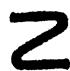
\includegraphics[keepaspectratio]{images/part002_cfff7d82.jpg}}

族 \((x_{i})\) 可和的这一必要条件一般绝不是充分的，即使 \(G\) 是完备的也是如此；后面我们会看到许多例子（见第四章，§ 7）。

推论. 设 \((x_{t})_{t\in I}\) 是交换群中的可和族，且该群的单位元有可数基本邻域系。那么指标 \(\iota\) 中使 \(x_{\iota}\neq 0\) 的那些组成的集合是可数的。

设 \((\mathbf{V}_{n})\) 是 0 的可数基本邻域系。若 \(\mathbf{H}_{n}\) 是使 \(x_{i} \notin \mathbf{V}_{n}\) 的所有指标 i 组成的集合，则使 \(x_{i} \neq 0\) 的指标 i 组成的集合 H 是诸集合 \(\mathbf{H}_{n}\) 的并，而由命题 1，每个 \(\mathbf{H}_{n}\) 都是有限的。

如果我们不假设原点有可数基本邻域系，这个推论就未必再成立。* 例如考虑积群 \(\mathbf{R}^{\mathbb{R}}\){[}实变量的所有有限实值函数作成的加法群，赋以逐点收敛拓扑（参看第十章，§ 1，第 3 节）{]}，并设 \(f_{a}\) 是 \(\mathbf{R}\) 中满足 \(f_{a}(a)=1\) 且 \(f_{a}(x)=0\)（当 \(x\neq a\) 时）的元素；那么族 \((f_{a})_{a\in\mathbb{R}}\) 是可和的，其和是在 \(\mathbf{R}\) 的每点取值都为 1 的函数。 *

注. 当 G 写作乘法时，Cauchy 判别准则取如下形式：为使族 \((x_{i})_{i\in I}\) 可乘，必须对单位元的每个邻域 V，存在 I 的有限子集 \(J_{0}\)，使得对 I 的每个不与 \(J_{0}\) 相交的有限子集 K，都有 \(\prod_{i\in K}x_{i}\in V\)；而且只要 G 是完备的，这个条件也是充分的。由此推出，若 I 是无限集且 \((x_{i})\) 可乘，则关于 I 的有限子集的余集所成的滤子，有 \(\lim x_{i}=1\)；若此外单位元还有可数基本邻域系，则使 \(x_{i}\neq1\) 的指标 i 组成的集合是可数的。

\subsection{部分和；结合性}

命题 2. 在完备群 G 中，可和族的每个子族都是可和的。

因为若族 \((x_{i})_{i\in I}\) 满足 Cauchy 判别准则，那么它的每个子族都平凡地满足该准则。

因此，若 \((x_{i})_{i\in I}\) 可和，则和 \(\sum_{i\in J}x_{i}\) 对每个子集 \(J\)（\(I\) 的，无论有限与否）都有定义：我们仍称它为族 \((x_{i})\) 的对应于指标集的子集 \(J\) 的部分和。可和族的部分和全体显然包含在有限部分和全体的闭包中。

定理 2（和的结合性）. 设 \((x_{i})_{i\in I}\) 是完备群 \(\mathbf{G}\) 中的可和族，并设 \((I_{\lambda})_{\lambda \in L}\) 是 \(\mathbf{I}\) 的任意一个分拆。若用 \(s_{\lambda}\) 表示 \(\sum_{i\in I_{\lambda}}x_{i}\)，则族 \((s_{\lambda})_{\lambda \in L}\) 可和且与族 \((x_{i})_{i\in I}\) 有相同的和。

设 \(s = \sum_{i \in I} x_i\)，并设 \(V\) 是 \(G\) 中 0 的任意闭邻域。那么存在有限子集 \(J_0\)（含于 \(I\)），使得对每个有限子集 \(J\)（含于 \(I\) 且包含 \(J_0\)），都有 \(\sum_{i \in J} x_i \in s + V\)。设 \(K_0\) 是 \(L\) 的由这样的指标 \(\lambda\) 组成的子集：它们使 \(J_\lambda = I_\lambda \cap J_0\) 非空；\(K_0\) 显然是有限的。设 \(K\) 是 \(L\) 的包含 \(K_0\) 的任意有限子集；我们将证明 \(\sum_{\lambda \in K} s_\lambda \in s + V\)，由此即证得定理。现在，\(s_\lambda\) 与 \((x_i)\) 的某个指标全属于 \(I_\lambda\) 的有限部分和非常接近；更精确地说，给定 0 的任意对称邻域 \(W\)，对每个 \(\lambda \in K\) 存在有限子集 \(H_\lambda\)（含于 \(I_\lambda\)，包含 \(J_\lambda\)），使得 \(s_\lambda - \sum_{i \in H_\lambda} x_i \in W\)。令 \(J = \bigcup_{\lambda \in K} H_\lambda\)；则 \(J\) 是 \(I\) 的包含 \(J_0\) 的有限子集，并且我们有

\[
\sum_ {i \in J} x _ {i} = \sum_ {\substack {i \in \bigcup_ {\lambda \in K} H _ {\lambda}}} x _ {i} = \sum_ {\lambda \in K} (\sum_ {i \in H _ {\lambda}} x _ {i})
\]

这是由有限和的结合性得到的。于是，由于 \(J_{0}\) 与诸 \(H_{\lambda}\) 的取法，我们有

\[
\sum_ {\lambda \in \mathbf {K}} s _ {\lambda} \in s + \mathbf {V} + n \mathbf {W}
\]

其中 \(n\) 是 \(\mathbf{K}\) 中元素的个数；这个关系式对每个 \(\mathbf{W}\) 都成立，从而也有 \(\sum_{\lambda \in \mathbb{K}} s_{\lambda} \in s + \mathbf{V}\)，因为 \(\mathbf{V}\)（是闭的）是诸邻域 \(\mathbf{V} + n\mathbf{W}\) 的交{[}§ 3，第 1 节，公式 (1){]}。

于是我们可以写出和的结合公式：

\[
\sum_ {\lambda \in L} (\sum_ {i \in I _ {\lambda}} x _ {i}) = \sum_ {i \in \bigcup_ {\lambda \in L} I _ {\lambda}} x _ {i},\tag{1}
\]

只要族 \((I_{\lambda})\) 是其并集的一个分拆且右端有定义，这个公式就成立。特别地，若指标集是积 \(I = L \times M\)，且“双重”族 \((x_{\lambda\mu})_{(\lambda,\mu) \in L \times M}\) 可和，我们就有求和次序交换的公式

\[
\sum_ {(\lambda , \mu) \in \mathbf {L} \times \mathbf {M}} x _ {\lambda \mu} = \sum_ {\lambda \in \mathbf {L}} (\sum_ {\mu \in \mathbf {M}} x _ {\lambda \mu}) = \sum_ {\mu \in \mathbf {M}} (\sum_ {\lambda \in \mathbf {L}} x _ {\lambda \mu}).\tag{2}
\]

应当指出，(1) 的左端可以有意义，而右端却没有定义。例如考虑 \(I = L \times \{1, 2\}\) 且 L 是无限集、\(I_{\lambda}\) 由 \((\lambda, 1)\) 与 \((\lambda, 2)\) 两个元素组成的情形；若取 \(x_{\lambda,1} = a\)，\(x_{\lambda,2} = -a\)，其中 \(a\) 是 \(\mathbf{G}\) 的任意非零元素，则对应于诸 \(I_{\lambda}\) 的所有部分和都为零，因此 (1) 的左端有定义且等于 0，而由命题 1，(1) 的右端没有意义。

同样可能发生这样的情形：(2) 的左端没有定义，但 (2) 中的两个“双重和”却都有意义；并且它们所表示的 G 的元素未必相等（见第四章，§ 7，习题 17）。

因此，虽然总是可以把一个和的项“结合”起来，但反过来却不可能把和式中本身表现为和的那些项“分解”为它们的元素。不过，只要这些“可分解”项的数目是有限的，这个运算就是合法的。

命题 3. 设 \((x_{\iota})_{\iota \in \mathbf{I}}\) 是群 \(\mathbf{G}\) 的点族，\((I_{\lambda})_{\lambda \in \mathbf{L}}\) 是 \(\mathbf{I}\) 的有限分拆。若每个子族 \((x_{\iota})_{\iota \in \mathbf{I}_{\lambda}}\) 都可和，则族 \((x_{\iota})_{\iota \in \mathbf{I}}\) 可和且公式 (1) 成立。

只需对 \(L = (1,2)\) 的情形证明本命题；在此基础上，再对 L 的元素个数用归纳法进行。设 \(s_{1} = \sum_{i \in I_{1}} x_{i}\)，\(s_{2} = \sum_{i \in I_{2}} x_{i}\)。对原点的每个邻域 V，存在有限子集 \(J_{1}\)（相应地，\(J_{2}\)），它含于 \(I_{1}\)（相应地，\(I_{2}\)），使得对每个有限子集 \(H_{1}\)（相应地，\(H_{2}\)）——含于 \(I_{1}\)（相应地，\(I_{2}\)）且包含 \(J_{1}\)（相应地，\(J_{2}\)）——有 \(\sum_{i \in H_{1}} x_{i} \in s_{1} + V\)（相应地，\(\sum_{i \in H_{2}} x_{i} \in s_{2} + V\)）。若令 \(J_{0} = J_{1} \cup J_{2}\)，则由此推出，对 I 的包含 \(J_{0}\) 的每个有限子集 H，有 \(\sum_{i \in H} x_{i} \in s_{1} + s_{2} + V + V\)，结论得证。

\subsection{群的积中的可和族}

命题 4. 设 \(G = \prod_{\lambda \in L} G_{\lambda}\) 是一族豪斯多夫交换群的积。那么诸点 \((x_{i})_{i \in I}\)（\(G\) 的点）构成的族可和当且仅当对每个 \(\lambda \in L\)，族 \((\mathbf{pr}_{\lambda} x_{i})_{i \in I}\) 可和；且若 \(s_{\lambda}\) 是这个族的和，则 \(s = (s_{\lambda})\) 是族 \((x_{i})\) 的和。

这由取值于积空间的函数关于滤子收敛的条件（第一章，§ 1，第 6 节，命题 10 的推论 1）立即得出；实际上，对 I 的每个有限子集 J，我们有

\[
\mathrm{pr} _ {\lambda} \left(\sum_ {i \in J} x _ {i}\right) = \sum_ {i \in J} \mathrm{pr} _ {\lambda} x _ {i}.
\]

\subsection{可和族在连续同态下的像}

命题 5. 设 \(f\) 是交换群 \(G\) 到交换群 \(G'\) 中的连续同态。若 \((x_t)\) 是 \(G\) 中的可和族，则 \((f(x_t))\) 是 \(G'\) 中的可和族，并且我们有

\[
\Sigma f (x _ {i}) = f (\Sigma x _ {i}).\tag{3}
\]

若 J 是指标集的任意有限子集，则 \(f\left(\sum_{i \in \mathbb{J}} x_i\right) = \sum_{i \in \mathbb{J}} f(x_i)\)，且收敛滤子基在 f 下的像是收敛滤子基（第一章，§ 7，第 4 节，命题 9 的推论 1）。

命题 6. 设 \((x_{i}), (y_{i})\) 是群 G 中有同一指标集的两个可和族。那么族 \((-x_{i}), (nx_{i})\)（ \(n \in \mathbf{Z}\)），\((x_{i} + y_{i})\) 都可和，并且我们有

\begin{enumerate}
\def\labelenumi{(\arabic{enumi})}
\setcounter{enumi}{3}
\tightlist
\item
\end{enumerate}

\[
\Sigma (- x _ {i}) = - \Sigma x _ {i},\tag{5}
\]

\[
\Sigma (n x _ {i}) = n \Sigma x _ {i},\tag{6}
\]

\[
\Sigma (x _ {i} + y _ {i}) = \Sigma x _ {i} + \Sigma y _ {i}.
\]

因为 \(x \rightarrow -x\) 与 \(x \rightarrow nx\) 都是 G 到 G 中的连续同态；另一方面，若 \((x_{t})\) 与 \((y_{t})\) 可和，则族 \((x_{t}, y_{t})\) 在 \(G \times G\) 中可和，且由于 \((x, y) \rightarrow x + y\) 是 \(G \times G\) 到 G 中的连续同态，我们即得 (6)。

注. 命题 4 与命题 5 也适用于前面提到过的情形，即具有一个结合且交换的合成法则的拓扑空间 X 中的可和族；若再假设 \(x + y\) 在 \(X \times X\) 上连续，则命题 3 与公式 (6) 也同样适用。

\subsection{级数}

考虑豪斯多夫交换群中的点列 \((x_{n})_{n\in \mathbb{N}}\)，并作部分和序列 \(s_n = \sum_{p=0}^{n} x_p (n \in \mathbb{N})\)。映射 \((x_{n}) \to (s_{n})\) 是集合 \(\mathbf{G}^{\mathbf{N}}\)（即点列 \((x_{n})\)（\(\mathbf{G}\) 中的）的全体）到其自身上的双射；因为若给定了序列 \((s_{n})\)，则序列 \((x_{n})\) 由关系 \(x_{0} = s_{0}, x_{n} = s_{n}-s_{n-1} (n \geqslant 1)\) 确定。

由序列 \((x_{n})\) 所定义的级数，或通项为 \(x_{n}\) 的级数{[}在不致混淆时，按用语之便，径称级数 \((x_{n})\){]}，定义为如上相关联的序列偶 \((x_{n})\) 与 \((s_{n})\)。由序列 \((x_{n})\) 所定义的级数称为收敛的，如果序列 \((s_n)\) 收敛；这个序列的极限称为级数的和，记作 \(\sum_{n=0}^{\infty} x_n\)（按记号之便，或记 \(\sum_{n=0}^{\infty} x_n\)）。

若通项为 \(x_{n}\) 的级数收敛，我们有时会按用语之便，称它为“级数 \(\sum_{n=0}^{\infty} x_{n}\)”或“级数 \(x_{0} + x_{1} + \cdots + x_{n} + \cdots\)”。

通项为 \(x_{n}\) 的级数收敛的一个必要条件是序列 \((s_{n})\) 为 Cauchy 序列，也就是说，对 G 中原点的每个邻域 V，存在整数 \(n_{0}\)，使得对每对整数 \(n \geqslant n_{0}, p > 0\)，有

\[
s _ {n + p} - s _ {n} = \sum_ {i = n + 1} ^ {n + p} x _ {i} \in V.
\]

若 \(\mathbf{G}\) 是完备的，这个条件也是充分的（级数的 Cauchy 判别准则）。

若通项为 \(x_{n}\) 的级数收敛，特别地我们有 \(\lim_{n\to \infty}(s_n - s_{n-1}) = \lim_{n\to \infty}x_n = 0\)；但这个收敛的必要条件一般绝不是充分的，即使 \(G\) 是完备的也是如此（见第四章，§ 7）。

命题 7. 若由序列 \((x_{n})\) 与 \((y_{n})\) 所定义的级数都收敛，则由序列 \((-x_{n})\) 与 \((x_{n} + y_{n})\) 所定义的级数也收敛，并且我们有

\[
\sum_ {n = 0} ^ {\infty} (- x _ {n}) = - \sum_ {n = 0} ^ {\infty} x _ {n},\tag{7}
\]

\[
\sum_ {n = 0} ^ {\infty} \left(x _ {n} + y _ {n}\right) = \sum_ {n = 0} ^ {\infty} x _ {n} + \sum_ {n = 0} ^ {\infty} y _ {n}.\tag{8}
\]

这是 \(-x\) 在 \(\mathbf{G}\) 上连续以及 \(x + y\) 在 \(\mathbf{G} \times \mathbf{G}\) 上连续的一个明显推论。

推论. 若 \((x_{n})\)、\((y_{n})\) 是 G 的两个点序列，使得除有限个指标外都有 \(x_{n}=y_{n}\)，且通项为 \(x_{n}\) 的级数收敛，则通项为 \(y_{n}\) 的级数也收敛。

因为通项为 \(x_{n} - y_{n}\) 的级数从某个指标起各项皆为零。

这个推论可以表述为：我们可以任意改动收敛级数的有限个项而不使它失去收敛性。特别地，若 \(y_{n} = 0\)（对 \(n < m\)），且 \(y_{n} = x_{n}\)（对 \(n \geqslant m\)），

则我们看到通项为 \(y_{n}\) 的级数收敛当且仅当通项为 \(x_{n}\) 的级数收敛；其和记作 \(\sum_{n=m}^{\infty} x_{n}\)，称为指标为 \(m\) 的余项（级数 \((x_{n})\) 的余项）。由于

\[
\sum_ {n = m} ^ {\infty} x _ {n} = \sum_ {n = 0} ^ {\infty} x _ {n} - s _ {m - 1},
\]

收敛级数的第 \(m\) 余项当 \(m\) 趋于 \(+\infty\) 时趋于 o。

若序列 \((x_{n})_{n\in I}\) 的指标集是 \(I\)——\(N\) 的无限子集——，且 \(\varphi\) 表示 \(N\) 到 \(I\) 上的保持严格序的双射，则按用语之便，称由序列 \((x_{\varphi(n)})_{n\in N}\) 所定义的级数为由序列 \((x_{n})_{n\in I}\) 所定义的级数；若这个级数收敛，其和记作 \(\sum_{n\in I}x_n\)。立即可以验证，这个级数收敛当且仅当通项为 \((z_n)\) 的级数收敛，其中 \(z_{n}=x_{n}\)（若 \(n\in I\)），而 \(z_{n}=0\)（若 \(n\in G I\)）。

\pandocbounded{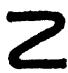
\includegraphics[keepaspectratio]{images/part002_ebf593f8.jpg}}

值得注意的是，若由序列 \((x_{n})_{n\in \mathbb{N}}\) 所定义的级数收敛，仍可能存在 \(\mathbf{N}\) 的无限子集 I，使得由子列 \((x_{n})_{n\in \mathbb{I}}\) 所定义的级数不收敛（见习题 5 及第四章，§ 7）。

命题 4 与命题 5 立即推广到级数，我们把它们在这一情形的表述留给读者。

命题 8（级数的受限结合性）. 设 \((k_n)\) 是一个严格递增的整数序列（\(\geqslant 0\)）。若通项为 \(x_n\) 的级数收敛，且令 \(u_n = \sum_{p=k_{n-1}}^{k_n-1} x_p\)，则通项为 \(u_n\) 的级数收敛，且我们有 \(\sum_{n=0}^{\infty} u_n = \sum_{n=0}^{\infty} x_n\)。

因为级数 \((u_{n})\) 的部分和序列是一个子列 \((s_{k_{n}-1})\)，它取自部分和序列 \((s_{n})\)（级数 \((x_{n})\) 的部分和序列）。

\subsection{交换收敛级数}

设 \((x_{n})\) 是 \(G\) 中的可和序列，并设 \(s = \sum_{n\in \mathbb{N}}x_n\) 是它的和。那么对每个邻域 \(V\)（\(0\) 的邻域），存在 \(J_0\in \mathfrak{F}(N)\)，使得 \(s_J\in s + V\) 只要 \(J\in \mathfrak{F}(N)\) 且 \(J_0\subset J\)。设 \(m\) 是 \(J_0\) 中最大的整数；则当 \(n\geqslant m\) 时有 \(s_n\in s + V\)，因而级数 \((x_{n})\) 收敛且其和为 \(s\)。但反之不成立：

收敛级数的项所成的序列完全可能不是可和的（见第四章，§ 7）。

此外，收敛级数的定义本质上涉及 N 的序结构。若级数 \((x_{n})\) 收敛，且 \(\sigma\) 是 N 的一个置换，则级数 \((x_{\sigma(n)})\) 未必收敛（参见第四章，§ 7，习题 15）。

定义 2. 由序列 \((x_{n})\) 所定义的级数称为交换收敛的，如果对每个置换 \(\sigma\)（\(\mathbf{N}\) 的置换），由序列 \((x_{\sigma(n)})\) 所定义的级数都收敛。

命题 9. 由序列 \((x_{n})\) 所定义的级数交换收敛当且仅当序列 \((x_{n})\) 可和；且此时对每个置换 \(\sigma\)（\(\mathbf{N}\) 的置换），我们有

\[
\sum_ {n = 0} ^ {\infty} x _ {\sigma} = \sum_ {n \in \mathbb {N}} x _ {n}.
\]

若序列可和，则级数显然交换收敛。为证反向的蕴含关系，我们用反证法，设级数 \((x_{n})\) 交换收敛而序列 \((x_{n})\) 不可和。于是滤子 \(\Phi\) 在映射 \(\mathbf{H} \to s_{\mathbf{H}}\) 下的像不能是 \(\mathbf{G}\) 中的 Cauchy 滤子基，否则这个滤子基将收敛，因为按假设它有一个聚点（第二章，§ 3，第 2 节，命题 5，推论 2）。因此存在一个邻域 \(\mathbf{V}\)（\(o\) 在 \(\mathbf{G}\) 中的一个邻域），使得对每个有限子集 \(\mathbf{J}\)（\(\mathbf{N}\) 的有限子集），存在有限子集 \(\mathbf{H}\)（\(\mathbf{N}\) 的有限子集），它不与 \(\mathbf{J}\) 相交，且使得 \(\sum_{n \in \mathbf{H}} x_{n} \notin V\)。于是，用归纳法，我们可以定义

把 N 分拆为有限子集 \(H_{k}\)（ \(k \in N\)），使得对无穷多个指标 k 有 \(\sum_{n \in H_{k}} x_{n} \notin V\)。显然存在 N 的一个置换 \(\sigma\)，使得对每个 k，使 \(\sigma(n) \in H_{k}\) 的那些 n 的值是相继的。若 \(\sigma\) 是这样一个置换，则通项为 \(x_{\sigma(n)}\) 的级数不可能收敛，于是得到矛盾。

若群 G 写作乘法，由 G 的点的序列 \((x_{n})\) 所定义的无穷乘积（或通项为 \(x_{n}\) 的无穷乘积，甚或在无混淆之虞时径称乘积 \(x_{n}\)）定义为序列 \((x_{n})\) 与部分积序列 \(p_{n}=\prod_{k=0}^{n}x_{k}\) 所构成的偶。若序列 \((p_{n})\) 收敛，则称该无穷乘积收敛，这个序列的极限记作 \(\prod_{n=0}^{\infty}x_{n}\)（按记号之便，或记 \(\prod_{n=0}^{\infty}x_{n}\)）。我们把将已建立的级数性质改写为乘法记号的任务留给读者。

\section{带算子拓扑群；拓扑环、除环与域}

\subsection{带算子拓扑群}

在集合 G 上，带算子的群结构与一个拓扑称为相容的，如果 G 的拓扑与群结构相容（§ 1，第 1 节），并且此外由算子所产生的 G 的自同态都是连续的。这时，集合 G 连同所给的拓扑与带算子的群结构，称为一个带算子拓扑群。

若 H 是带算子拓扑群 G 的稳定子群，则由 G 的拓扑在 H 上诱导的拓扑与 H 上的带算子群结构相容。此外：

命题 1. 若 H 是带算子拓扑群 G 的稳定子群，则 H 在 G 中的闭包 \(\overline{H}\) 是 G 的稳定子群。

我们已知（§ 2，第 1 节，命题 1）\(\overline{\mathbf{H}}\) 是 G 的子群。又若 \(\alpha\) 是 G 上的任一算子，则 H 在连续映射 \(x \to x^{\alpha}\) 下的像含于 H，因而 \(\overline{\mathbf{H}}\) 的像含于 \(\overline{\mathbf{H}}\)（第一章，§ 2，第 1 节，定理 1）。

设 H 是带算子拓扑群 G 的稳定正规子群。那么对 G 上的每个算子 \(\alpha\)，由 \(x \rightarrow x^{\alpha}\) 诱导的 G/H 到其自身的映射是连续的（§ 2，第 8 节，注 3），因此 G/H 上的带算子群结构与 G/H 上的商拓扑相容。

设 \((\mathbf{G}_i)_{i\in I}\) 是带算子拓扑群的一个族，其中假定每个 \(\mathbf{G}_i\) 有同一个算子集 \(\Omega\)。对每个 \(\alpha \in \Omega\)，映射 \(x\to ((\mathrm{pr}_i x)^{\alpha})\)（\(\mathbf{G} = \prod_{i\in I}\mathbf{G}_i\) 到其自身的映射）是连续的（第一章，§ 4，第 1 节，命题 1），因此 \(\mathbf{G}\) 上的带算子群结构与 \(\mathbf{G}\) 上的积拓扑相容。

若 G 是带算子的豪斯多夫拓扑群且 G 有完备化 \(\hat{G}\)（§ 3，第 4 节），则 G 上由算子定义的每个自同态 \(x \to x^{\alpha}\) 都可由连续性延拓为 \(\hat{\mathbf{G}}\) 的自同态（§ 3，第 3 节，命题 5）。于是 \(\hat{\mathbf{G}}\) 具有带算子拓扑群的结构，且 \(\hat{\mathbf{G}}\) 与 \(\mathbf{G}\) 有同一个算子集。

\subsection{稳定子群的拓扑直和}

由于带算子交换群的研究等同于模的研究，我们有时会容许自己对任意的带算子交换群使用专属于模的术语；这样，我们可以用线性映射一词来代替带算子交换群的同态，并可用投影算子一词来指带算子交换群的幂等自同态。

若带算子的交换拓扑群 \(\mathbf{E}\)（写作加法）是稳定子群的一个有限族 \((\mathbf{M}_i)_{1 \leqslant i \leqslant n}\) 的直和，则典范双射 \((x_i) \to \sum_{i=1}^{n} x_i\)（积群 \(\prod_{i=1}^{n} \mathbf{M}_i\) 到 \(\mathbf{E}\) 上的双射）是连续的，但未必是同胚。

定义 1. 设 E 是带算子的交换拓扑群，并设 \((\mathbf{M}_i)_{1 \leqslant i \leqslant n}\) 是 E 的稳定子群的一个有限族，使 E 是诸 \(\mathbf{M}_i\) 的直和。当下述条件成立时称 E 是诸 \(\mathbf{M}_i\) 的拓扑直和：典范映射 \((x_i) \to \sum_{i=1}^{n} x_i\)（积群 \(\prod_{i=1}^{n} \mathbf{M}_i\) 到 E 上的映射）是一个同胚（从而是带算子拓扑群的一个同构）。

命题 2. 设 E 是带算子的交换拓扑群，它是稳定子群 \(\mathbf{M}_i\)（ \(1 \leqslant i \leqslant n\)）的直和。设 \((p_i)_{1 \leqslant i \leqslant n}\) 是与分解 \(\mathbf{E} = \sum_{i=1}^{n} \mathbf{M}_i\) 相伴随的投影算子族。则 E 是诸 \(\mathbf{M}_i\) 的拓扑直和当且仅当诸 \(p_i\) 连续。

因为映射 \(x \to (p_i(x))\) 是映射 \((x_i) \to \sum_{i=1}^{n} x_i\) 的逆。

由于 \(\mathbf{I} = \sum_{i=1}^{n} p_i\)（其中 \(\mathbf{I}\) 表示 \(\mathbf{E}\) 的恒等映射），只需 \(n - \mathbf{I}\) 个投影算子 \(p_i\) 连续，便足以保证第 \(n\) 个也连续。

若 E 是两个稳定子群 M、N 的拓扑直和，则称 N 是 M 在 E 中的拓扑补；此事成立当且仅当 E/M 到 N 上的典范映射是带算子拓扑群的一个同构。

推论. 设 E 是带算子的交换拓扑群，并设 M 是 E 的稳定子群。那么下列条件等价：

\begin{enumerate}
\def\labelenumi{\alph{enumi})}
\item
  M 在 E 中有一个拓扑补。
\item
  存在连续投影算子 \(p\)（\(\mathbf{E}\) 到 \(\mathbf{E}\) 中的投影算子），使得 \(p(\mathbf{E}) = \mathbf{M}\)。
\item
  M 的恒等映射可以延拓为 E 到 M 上的一个连续线性映射。
\end{enumerate}

由命题 2 推出 a) 蕴含 b)，而 b) 蕴含 c) 是显然的。最后，若 p 是 E 到 M 上的一个连续线性映射，它延拓 M 的恒等映射，则 p 是一个连续投影算子，且投影算子 p 与 1-p 相伴于直和分解 \(E = M + N\)，其中 \(N = p^{-1}(\mathbf{o})\)。

注. 1) 为避免混淆，我们有时把 E 的作为 M 的补（就带算子群结构而言，不涉及拓扑）的稳定子群称为 M 的代数补。

\begin{enumerate}
\def\labelenumi{\arabic{enumi})}
\setcounter{enumi}{1}
\tightlist
\item
  若带算子的豪斯多夫交换拓扑群是稳定子群的一个族 \((\mathbf{M}_i)_{1\leqslant i\leqslant n}\) 的拓扑直和，则每个子群 \(\mathbf{M}_i\) 在 E 中闭，因为 \(\mathbf{M}_i\) 是由所有这样的 \(x\in E\) 组成的集合：它们满足 \(p_i(x) = x\)（第一章，§ 8，第 1 节，命题 2）。
\end{enumerate}

命题 3. 设 E、F 是两个带算子的交换拓扑群，并设 u 是 E 到 F 中的一个连续线性映射。为使存在 F 到 E 中的一个连续线性映射 v，使得 \(u \circ v\) 是 F 的恒等映射（这时称 u 为右可逆，称 v 为 u 的一个右逆），必须且只需 u 是 E 到 F 上的一个严格态射（§ 2，第 8 节），且 \(u^{-1}(\mathbf{o})\) 在 E 中有一个拓扑补。

这些条件是必要的。因为这时有 \(u(v(\mathbf{F})) = \mathbf{F}\)，并且 \(a\) fortiori（更有）\(u(\mathbf{E}) = \mathbf{F}\)；此外，若 \(p = v \circ u\)，则 \(p\) 是 \(\mathbf{E}\) 到其自身中的一个连续线性映射，满足 \(p^2 = p\)；因此（命题 2 的推论）\(p(\mathbf{E}) = v(u(\mathbf{E})) = v(\mathbf{F})\) 有一个拓扑补 \(p^{-1}(\mathbf{o})\)（在 \(\mathbf{E}\) 中的）；但按假设 \(u(p(x)) = u(x)\)，我们有 \(u^{-1}(\mathbf{o}) = p^{-1}(\mathbf{o})\)。最后，\(\mathrm{E}/p^{-1}(\mathbf{o})\) 到 \(\mathbf{F}\) 上的双射（与 \(u\) 相伴的双射），是如下两个映射的复合：\(\mathrm{E}/u^{-1}(\mathbf{o})\) 到 \(v(\mathbf{F})\) 上的双射（与 \(p\) 相伴的双射），以及 \(u\) 在 \(v(\mathbf{F})\) 上的限制；由于 \(v\) 连续，这两个映射都是同构，因此 \(u\) 是 \(\mathbf{E}\) 到 \(\mathbf{F}\) 上的一个严格态射。

这些条件是充分的。因为若 \(\varphi\) 是 E 到 \(\mathrm{E}/u^{-1}(\mathbf{o})\) 上的典范同态，则说 \(u^{-1}(\mathbf{o})\) 在 E 中有一个拓扑补 M，就等于说 \(\varphi\) 在 M 上的限制是 M 到 \(\mathrm{E}/u^{-1}(\mathbf{o})\) 上的一个同构。另一方面，由于 \(u=w\circ\varphi\)，其中 w 是 \(\mathrm{E}/u^{-1}(\mathbf{o})\) 到 F 上的一个同构，可见 u 在 M 上的限制是 M 到 F 上的一个同构，因而逆同构 v 使得 \(u\circ v\) 是 F 到其自身的恒等映射。

命题 4. 设 E、F 是两个带算子的交换拓扑群，并设 u 是 E 到 F 中的一个连续线性映射。为使存在 F 到 E 中的一个连续线性映射 v，使得 \(v \circ u\) 是 E 到其自身的恒等映射（这时称 u 为左可逆，称 v 为 u 的一个左逆），必须且只需 u 是 E 到 u(E) 上的一个（拓扑）同构，且 u(E) 在 F 中有一个拓扑补。

这些条件是充分的，因为若它们满足，就得到一个左逆 \(v\)（\(u\) 的左逆），其做法是把 \(u(\mathbf{E})\) 到 \(\mathbf{E}\) 上的同构（即 \(u\) 的逆）与 \(\mathbf{F}\) 到 \(u(\mathbf{E})\) 上的一个连续投影算子复合。

这些条件是必要的。因为关系 \(v(u(x)) = x\) 表明 \(u^{-1}(\mathbf{o}) = \{0\}\)；于是 \(u\) 是 \(E\) 到 \(u(E)\) 上的一个双射，且由于 \(v\) 在 \(u(E)\) 上的限制连续，由此得出 \(u\) 是 \(E\) 到 \(u(E)\) 上的一个同构。另一方面，若令 \(q = u \circ v\)，则 \(q\) 是 \(F\) 到 \(u(E)\) 上的一个连续线性映射，满足 \(q^2 = q\)，这就证明（命题 2 的推论）\(u(E)\) 在 \(F\) 中有一个拓扑补。

\subsection{拓扑环}

定义 2. 拓扑环是一个集合 A，其上带有环结构与一个拓扑，满足下列公理：

\((\mathrm{AT}_{\mathbf{I}})\). 映射 \((x,y) \to x + y\)（\(\mathbf{A} \times \mathbf{A}\) 到 \(\mathbf{A}\) 中的映射）是连续的。

\((\mathrm{AT}_{\mathbf{II}})\). 映射 \(x \to -x\)（A 到 A 中的映射）是连续的。

\((\mathrm{AT}_{\mathrm{III}})\). 映射 \((x,y)\to xy\)（\(\mathbf{A}\times \mathbf{A}\) 到 \(\mathbf{A}\) 中的映射）是连续的。

前两条公理表明 \(\mathbf{A}\) 的拓扑与其加法群结构相容（§ 1，第 1 节）。

若在集合 A 上给定了环结构与一个拓扑，则当它们满足公理 \((\mathrm{AT}_{\mathbf{I}})\)、\((\mathrm{AT}_{\mathbf{II}})\) 与 \((\mathrm{AT}_{\mathbf{III}})\) 时，称它们是相容的。

例. 1) 在任一环 A 上，离散拓扑与环结构相容。拓扑为离散的拓扑环称为离散环。

* 2) 我们将在第四章看到，有理直线 Q（相应地，实直线 R）的拓扑与 Q（相应地，R）的环结构相容。 *

在拓扑环中，每个左位似 \(x \rightarrow ax\)（相应地，每个右位似 \(x \rightarrow xa\)）都是连续的（且当 a 是 A 的单位时是同胚）。

由于我们可以恒等地写出

\[
x y - x _ {0} y _ {0} = (x - x _ {0}) (y - y _ {0}) + (x - x _ {0}) y _ {0} + x _ {0} (y - y _ {0})
\]

公理 \((\mathrm{AT}_{\mathrm{III}})\){[}结合 \((\mathrm{AT}_{\mathrm{I}})\) 与 \((\mathrm{AT}_{\mathrm{II}})\){]}就等价于下列两条公理的合取：

\((\mathrm{AT}_{\mathrm{III}a})\). 对任意 \(x_0\in \mathbf{A}\)，映射 \(x\to x_0x\) 与 \(x\rightarrow xx_0\) 在点 \(x = 0\) 连续

\((\mathrm{AT}_{\mathbf{III}\ b})\). 映射 \((x,y)\rightarrow xy\)（\(\mathbf{A}\times \mathbf{A}\) 到 A 中的映射）在点 (o, o) 连续。

由此我们可以导出一组充要条件，使滤子 \(\mathfrak{B}\)（\(o\) 在一个环 \(A\) 中的邻域滤子）必须满足它们，才能在 \(A\) 上定义一个与其环结构相容的拓扑：\(\mathfrak{B}\) 必须满足 § 1 的公理 \((\mathrm{GA}_{\mathrm{I}})\) 与 \((\mathrm{GA}_{\mathrm{II}})\)，并且还满足下列两条公理：

\((\mathrm{AV}_{1})\). 对所有 \(x_0\in \mathbf{A}\) 与所有 \(\mathbf{V}\in \mathfrak{B}\)，存在 \(\mathbf{W}\in \mathfrak{B}\)，使得 \(x_0\mathbf{W}\subset \mathbf{V}\) 且 \(\mathbf{W}x_0\subset \mathbf{V}\)

\((\mathrm{AV}_{\mathrm{II}})\). 对所有 \(\mathbf{V} \in \mathfrak{B}\)，存在 \(\mathbf{W} \in \mathfrak{B}\)，使得 \(\mathbf{WW} \subset \mathbf{V}\)。

注. 在分析中我们相当经常遇到满足公理 \((\mathrm{AT}_{\mathrm{I}})\)、\((\mathrm{AT}_{\mathrm{II}})\) 与 \((\mathrm{AT}_{\mathrm{III}a})\)，但不满足 \((\mathrm{AT}_{\mathrm{III}b})\) 的环。* 紧群上的测度环就是一个例子，其中乘法是卷积，拓扑是淡拓扑。 *

例 3). 设 \(\mathfrak{B}\) 是环 A 上的一个滤子基，由双边理想组成。\(\mathfrak{B}\) 是某个拓扑（与 A 的加法群结构相容的拓扑）的 o 的基本邻域系，且由 \((\mathrm{AV}_{\mathrm{I}})\) 与 \((\mathrm{AV}_{\mathrm{II}})\) 立即得出，这个拓扑与 A 的环结构相容。

设 X 是拓扑空间，f 与 g 是 X 到拓扑环 A 中的两个映射。若 f 与 g 在一点 \(x_{0} \in X\) 连续，则 \(f + g\)、-f 与 fg 在该点连续。由此得出，X 到 A 中的连续映射组成 X 到 A 的一切映射所成之环 \(A^{X}\) 的一个子环。我们还看到，若 A 交换，则每个 n 个变元、系数在 A 中且定义在 \(A^{n}\) 上的多项式都在 \(A^{n}\) 上连续。再者，设 f 与 g 是一个集合 X（由滤子 F 所滤化）到豪斯多夫拓扑环 A 中的两个映射；若 \(\lim_{\mathfrak{F}} f\) 与 \(\lim_{\mathfrak{F}} g\) 存在，则 \(\lim_{\mathfrak{F}} (f + g)\)、\(\lim_{\mathfrak{F}} (-f)\) 与 \(\lim_{\mathfrak{F}} (fg)\) 也存在，并且我们有（第一章，§7，第 4 节，命题 9，推论 1，及 §8，第 1 节，命题 1）

\[
\lim _ {\mathfrak {F}} (f + g) = \lim _ {\mathfrak {F}} f + \lim _ {\mathfrak {F}} g,\tag{1}
\]

\[
\lim _ {\mathfrak {F}} (- f) = - \lim _ {\mathfrak {F}} f,\tag{2}
\]

\[
\lim _ {\mathfrak {F}} (f g) = (\lim _ {\mathfrak {F}} f) (\lim _ {\mathfrak {F}} g).\tag{3}
\]

\subsection{子环；理想；商环；环的积}

若 H 是拓扑环 A 的子环，则由 A 的拓扑在 H 上诱导的拓扑与 H 的环结构相容。这样在 H 上定义的拓扑环结构称为由 A 的拓扑环结构所诱导。

命题 5. 设 H 是拓扑环 A 的稠密子环，并设 K 是 H 的子环（相应地，左理想、右理想、双边理想）。则 K 在 A 中的闭包 K 是 A 的子环（相应地，左理想、右理想、双边理想）。

证明与 § 2 第 3 节命题 8 的证明相同：例如若 K 是 H 中的左理想，则映射 \((z, x) \to zx\) 在 \(A \times A\) 上连续，且把 \(H \times K\) 映入 K；因而它把 \(A \times K = \overline{H} \times K\) 映入 \(\overline{H}\)。

设 H 是拓扑环 A 中的双边理想。用与商群情形同样的论证，我们看到 A 的拓扑由关系 \(x - y \in H\) 作出的商与 A/H 的环结构相容。特别地，若 A 不是豪斯多夫的，则 \(\{o\}\) 在 A 中的闭包 N 由命题 5 是一个闭双边理想；商环是豪斯多夫的（§ 2，第 5 节，命题 13），称为与 A 相伴的 Hausdorff 环。

设 \((\mathbf{A}_t)_{t\in \mathbf{I}}\) 是拓扑环的一个族。在集合 \(\mathbf{A} = \prod_{t\in \mathbf{I}}\mathbf{A}_t\) 上，诸 \(\mathbf{A}_t\) 的拓扑之积与诸 \(\mathbf{A}_t\) 的环结构之积相容（与积群情形的证明相同）；这样定义的拓扑环 \(\mathbf{A}\) 称为诸拓扑环 \(\mathbf{A}_t\) 的积。

\subsection{拓扑环的完备化}

当我们说到拓扑环的一致结构时，除非另有明确说明，我们总是指其加法群的一致结构；特别地，若 A 的加法群完备，则称 A 为完备环。

设 A 是豪斯多夫拓扑环；作为加法群，A 可以看作完备豪斯多夫交换群 \(\hat{\mathbf{A}}\) 的一个稠密子群，后者在相差一个同构的意义下被确定（§ 3，第 5 节，定理 2）。为使我们可以把 A 看作完备环的子环，必须能够把函数 \(xy\) 由连续性延拓到空间 \(\hat{\mathbf{A}} \times \hat{\mathbf{A}}\) 上。这种延拓的可能性将由下面更一般的定理得出：

定理 1. 设 E、F、G 是三个完备豪斯多夫交换群；设 A 是 E 的稠密子群，B 是 F 的稠密子群。若 f 是 A × B 到 G 中的一个连续 Z-双线性（*）映射，则 f 可由连续性延拓为 E × F 到 G 中的一个连续 Z-双线性映射。

设 \((x_{0}, y_{0})\) 是 \(E \times F\) 的任意一点，并设 \(\mathfrak{U}\)、\(\mathfrak{B}\) 分别是 \(x_{0}, y_{0}\) 的邻域滤子在 A、B 上的迹（按假设 \(\mathfrak{U}\)、\(\mathfrak{B}\) 是滤子）。为证 f 可由连续性延拓，只需证明 \(f(\mathfrak{U} \times \mathfrak{V})\) 是 G 上的一个 Cauchy 滤子基（第二章，§ 3，第 6 节，命题 11）。考虑恒等式

\[
f \left(x ^ {\prime}, y ^ {\prime}\right) - f (x, y) = f \left(x ^ {\prime} - x, y _ {1}\right) + f \left(x _ {1}, y ^ {\prime} - y\right) + f \left(x ^ {\prime} - x, y ^ {\prime} - y _ {1}\right).
\]

我们将证明，取 \((x, y)\) 与 \((x', y')\) 属于 \(\mathfrak{U} \times \mathfrak{B}\) 的一个充分小的集合，并适当选取 \(x_{1}\) 与 \(y_{1}\)，就可以使右端各项都很小。设 W 是 G 中 o 的任一邻域；由于 f 在 \((o, o) \in A \times B\) 连续，存在集合 \(U \in \mathfrak{U}\) 与集合 \(V \in \mathfrak{B}\)，使得 \(f(x' - x, y' - y) \in W\) 对 \(x \in U\)、\(x' \in U\)、\(y \in V\)、\(y' \in V\) 均成立。取一点 \(x_{1} \in U\) 与一点 \(y_{1} \in V\)；则对 U 中所有 \(x, x'\) 与 V 中所有 \(y, y'\)，我们将有

\[
f \left(x ^ {\prime} - x, y ^ {\prime} - y _ {1}\right) + f \left(x - x _ {1}, y ^ {\prime} - y\right) \in \mathrm{W} + \mathrm{W}.
\]

另一方面，偏映射 \(x \to f(x, y_1)\) 在 A 上连续；因而存在集合 \(U' \subset U\)（属于 \(\mathfrak{U}\)），使得只要 \(x\) 与 \(x'\) 属于 \(U'\)，就有 \(f(x' - x, y_1) \in W\)。同样，存在 \(V' \subset V\)（属于 \(\mathfrak{B}\)），使得只要 \(y\) 与 \(y'\) 属于 \(V'\)，就有 \(f(x_1, y' - y) \in W\)。于是，若 \((x, y)\) 与 \((x', y')\) 是 \(U' \times V'\) 的任意两点，则

\[
f \left(x ^ {\prime}, y ^ {\prime}\right) - f (x, y) \in W + W + W + W;
\]

这就证明了延拓 \(\overline{f}\)（\(f\) 的延拓）的存在性。\(\overline{f}\) 是 \(\mathbf{Z}\)-双线性的这一事实，是恒等延拓原理（第一章，§ 8，第 1 节，命题 2 的推论 1）的直接推论。

证毕。

在把这一定理应用于豪斯多夫拓扑环 A 时，我们取 E、F 与 G 为 \(\hat{A}\)，取 A 与 B 为环 A，并取 f 为 Z-双线性映射 \((x, y) \to xy\)，按假设它是连续的。我们仍用 xy 表示延拓后的函数在 \(\hat{A} \times \hat{A}\) 上的值；这个函数是 \(\hat{A}\) 上的一个合成法则，说它是 Z-双线性的，就是说它关于加法双侧分配；又由恒等延拓原理，它也是结合的。于是：

命题 6. 豪斯多夫拓扑环 A 同构于完备豪斯多夫环 \(\hat{\mathbf{A}}\) 的一个稠密子环，后者在相差一个同构的意义下被确定（并称为 A 的完备化）。

若 A 交换（相应地，有单位元），则 \(\hat{A}\) 亦然（恒等延拓原理）。

设 A 是拓扑环，不必是豪斯多夫的；设 N 是 \(\{o\}\) 在 A 中的闭包，并设 \(A' = A/N\) 是与 A 相伴的 Hausdorff 环。则 \(\hat{A}'\)——\(A'\) 的完备化——称为 A 的 Hausdorff 完备化，也记作 \(\hat{A}\)。与 §3 第 4 节命题 8 一样可以证明，A 到完备豪斯多夫拓扑环 C 中的每个连续环同态 u 都可以唯一分解为 \(u = v \circ \varphi\)，其中 v 是 \(\hat{A}\) 到 C 中的连续同态，而 \(\varphi\) 是 A 到 \(\hat{A}\) 中的典范映射。若 A、B 是两个拓扑环，且 \(u : A \to B\) 是连续同态，则存在唯一的连续同态 \(\hat{u} : \hat{A} \to \hat{B}\)，使得图表

\[
\begin{array}{c c c} \mathbf {A} & \stackrel {{u}} {{\longrightarrow}} & \mathbf {B} \\ \varphi \Big \downarrow & & \Big \downarrow \psi \\ \hat {\mathbf {A}} & \stackrel {{\hat {u}}} {{\longrightarrow}} & \hat {\mathbf {B}} \end{array}
\]

是交换的（ \(\varphi\) 与 \(\psi\) 是典范映射）；只需对 \(\psi \circ u\) 应用前面的结果。

\subsection{拓扑模}

定义 3. 给定一个有单位元的拓扑环 A，拓扑左 A-模是一个集合 E，连同：

\begin{enumerate}
\def\labelenumi{\arabic{enumi})}
\item
  一个左 A-模结构；
\item
  一个与 E 的加法群结构相容的拓扑，且满足下列公理：
\end{enumerate}

(MT) 映射 \((\lambda, x) \to \lambda x\)（\(\mathbf{A} \times \mathbf{E}\) 到 \(\mathbf{E}\) 中的映射）是连续的。

我们类似地定义拓扑右 A-模的概念；由于每个右 A-模都可以看作左 A°-模（其中 A° 是 A 的反环），且 A 的拓扑与 A° 的环结构相容，因此无须区分拓扑右 A-模与拓扑左 A°-模。

例. *1) R（相应地，C）上的拓扑向量空间是拓扑 R（相应地，C）模。

\begin{enumerate}
\def\labelenumi{\arabic{enumi})}
\setcounter{enumi}{1}
\tightlist
\item
  设 A 是环，B 是 A 上由 A 的双边理想组成的一个滤子基；设 E 是左 A-模。若给 A 赋以 B 为 o 的基本邻域系的拓扑（与其环结构相容的拓扑）（第 3 节，例 3），并给 E 赋以诸集合 aE（当 a 取遍 B 时）构成 o 的基本邻域系的拓扑（与其加法群结构相容）（§ 1，第 2 节，例），则立即可以验证 E 是拓扑 A-模。
\end{enumerate}

注. 给定拓扑环 A，在左 A-模 E 上考虑一个与 E 的加法群结构相容的拓扑。凭恒等式

\[
\lambda x - \lambda_ {0} x _ {0} = (\lambda - \lambda_ {0}) x _ {0} + \lambda_ {0} (x - x _ {0}) + (\lambda - \lambda_ {0}) (x - x _ {0})
\]

公理 (MT) 等价于下列三条公理的合取：

\((\mathbf{MT}_{\mathbf{I}}^{\prime})\). 对每个 \(x_0\in \mathbf{E}\)，映射 \(\lambda \to \lambda x_0\) 在点 \(\lambda = 0\) 连续

\((\mathbf{MT}_{\mathrm{II}}^{\prime})\). 对每个 \(\lambda_0\in \mathbf{A}\)，映射 \(x\to \lambda_0x\) 在点 \(x = 0\) 连续

\((\mathbf{MT}_{\mathrm{III}}^{\prime})\). 映射 \((\lambda ,x)\to \lambda x\) 在点 (o, o) 连续。

由此我们导出一组充要条件，A-模 E 中 o 的邻域滤子 \(\mathfrak{B}\) 必须满足它们，才能在 E 上定义一个与其模结构相容的拓扑；\(\mathfrak{B}\) 必须满足 § 1 第 2 节的公理 (GA \(_{\mathrm{I}}\) ) 与 (GA \(_{\mathrm{II}}\) )，此外还必须满足下列三条公理：

\((\mathbf{MV}_{\mathrm{I}})\). 对每个 \(x_0 \in E\) 与 V \(\in \mathfrak{B}\)，存在 A 中 o 的一个邻域 S，使得 S. \(x_0 \subset V\)。

\((\mathbf{MV}_{\mathrm{II}})\). 对每个 \(\lambda_0 \in \mathbf{A}\) 与 \(V \in \mathfrak{B}\)，存在 \(W \in \mathfrak{B}\)，使得 \(\lambda_0 W \subset V\)。\((\mathbf{MV}_{\mathrm{III}})\). 对每个 \(V \in \mathfrak{B}\)，存在 \(U \in \mathfrak{B}\) 与一个邻域 \(T\)（\(o\) 在 \(A\) 中的一个邻域），使得 \(T. U \subset V\)。

当环 \(\mathbf{Z}\) 赋以离散拓扑时，每个交换拓扑群都是拓扑 \(\mathbf{Z}\)-模。

若 M 是拓扑 A-模 E 的子模，则显然由 E 的拓扑在 M 上诱导的拓扑与 M 的模结构相容。此外，在商 A-模 E/M 上，E 的拓扑对 M 作出的商拓扑与 A-模结构相容。为看清这一点，只需证明映射 \((\lambda, \dot{x}) \to \lambda \dot{x}\)（\(\mathbf{A} \times (\mathbf{E} / \mathbf{M})\) 到 \(\mathbf{E} / \mathbf{M}\) 上的映射）连续（其中 \(x \to \dot{x}\) 表示 \(\mathbf{E}\) 到 \(\mathbf{E} / \mathbf{M}\) 上的典范映射）。现在，由于我们可以把加法拓扑群 \(\mathbf{A} \times (\mathbf{E} / \mathbf{M})\) 与 \((\mathbf{A} \times \mathbf{E}) / (\{\mathbf{o}\} \times \mathbf{M})\) 等同起来（§ 2，第 9 节，命题 26 的推论），只需证明映射 \((\lambda, x) \to \lambda \dot{x}\)（\(\mathbf{A} \times \mathbf{E}\) 到 \(\mathbf{E} / \mathbf{M}\) 中的映射）连续；而这是直接的，因为所论映射是 \(x \to \dot{x}\) 与 \((\lambda, x) \to \lambda x\) 的复合。

设 \((\mathbf{E}_i)_{i\in \mathbf{I}}\) 是拓扑 A-模的任意一个族，并设 \(\mathbf{E} = \prod_{i\in \mathbf{I}}\mathbf{E}_i\) 是诸 \(\mathbf{E}_i\) 之积这个 A-模。则 E 上的

积拓扑与 E 的 A-模结构相容。为证明这一点，只需证明 A × E 到 E 中的映射 \((\lambda, x) \to (\lambda \cdot \text{pr}_i x)_{i \in I}\) 连续，或者（由第一章 § 4 第 1 节命题 1）对每个指标 \(i \in I\)，映射 \((\lambda, x) \to \lambda \cdot \text{pr}_i x\) 是 A × E 到 \(E_i\) 中的连续映射；但这个映射是 \((\lambda, x_i) \to \lambda x_i\) 与 \((\lambda, x) \to (\lambda, \text{pr}_i x)\) 的复合，而这两个映射都是连续的。

设 A 是豪斯多夫拓扑环，E 是豪斯多夫拓扑 A-模。设 \(\hat{\mathbf{E}}\) 是作为交换拓扑群 E 的完备化的那个加法群（§ 3，第 5 节，定理 2）。Z-双线性映射 \((\lambda, x) \to \lambda x\)（加法群 A、E 之积 \(\mathbf{A} \times \mathbf{E}\) 到加法群 E 中的映射）可由连续性延拓为 \(\hat{\mathbf{A}} \times \hat{\mathbf{E}}\) 到 \(\hat{\mathbf{E}}\) 中的 Z-双线性映射（第 5 节，定理 1），我们仍把这个映射记作 \((\lambda, x) \to \lambda x\)。由恒等延拓原理，我们有 \(\lambda(\mu x) = (\lambda \mu)x\)（对 \(\lambda \in \hat{\mathbf{A}}\)、\(\mu \in \hat{\mathbf{A}}\) 与 \(x \in \hat{\mathbf{E}}\)），且 \(1.x = x\) 对所有 \(x \in \hat{\mathbf{E}}\)；因此外合成法则 \((\lambda, x) \to \lambda x\) 所定义的 \(\hat{\mathbf{A}}\)-模结构在 \(\hat{\mathbf{E}}\) 上与它的拓扑相容。这样定义的拓扑 \(\hat{\mathbf{A}}\)-模 \(\hat{\mathbf{E}}\) 称为拓扑 A-模 E 的完备化。

设 E 是拓扑环 A 上的拓扑模，其中 A 与 E 都不必是豪斯多夫的。设 N（相应地，F）是 \(\{o\}\) 在 A（相应地，E）中的闭包。N 是 A 的双边理想（第 4 节，命题 5），F 是 E 的子 A-模（第 1 节，命题 1）；此外，由连续性我们有 \(\lambda x \in F\)，只要 \(\lambda \in N\) 或 \(x \in F\)。因此我们可以通过过渡到商来定义映射 \((\dot{\lambda}, \dot{x}) \to \dot{\lambda} \dot{x}\)（\((A/N) \times (E/F)\) 到 E/F 中的映射）；容易验证（利用 § 2 第 9 节命题 26 的推论）这个映射连续，从而在 E/F 上定义了一个拓扑 \((A/N)\)-模结构。若令 B = A/N 与 L = E/F，则 B-模 L 称为与 E 相伴的 Hausdorff 模；它的完备化 \(\hat{L}\) 是 \(\hat{A}\)——A 的 Hausdorff 完备化，按定义等于 \(\hat{B}\)——上的一个拓扑模（第 5 节），而这个模 \(\hat{L}\) 称为 E 的 Hausdorff 完备化，记作

\(\hat{\mathbf{E}}\)。与 § 3 第 4 节命题 8 一样可以看到，每个连续同态 \(u: \mathbf{E} \to \mathbf{G}\)（\(\mathbf{E}\) 到完备豪斯多夫 \(\hat{\mathbf{A}}\)-模 \(\mathbf{G}\) 中的连续同态）都唯一分解为 \(u = v \circ \varphi\)，其中 \(v\) 是 \(\hat{\mathbf{E}}\) 到 \(\mathbf{G}\) 中的连续同态，而 \(\varphi\) 是 \(\mathbf{E}\) 到 \(\hat{\mathbf{E}}\) 中的典范映射。我们断言，若 \(\mathbf{E}, \mathbf{E}'\) 是两个拓扑 A-模，且 \(u: \mathbf{E} \to \mathbf{E}'\) 是连续同态，则存在唯一的连续同态 \(\hat{u}: \hat{\mathbf{E}} \to \hat{\mathbf{E}}'\)，使得图表

\[
\begin{array}{c c c} \mathbf {E} & \stackrel {{u}} {{\longrightarrow}} & \mathbf {E} ^ {\prime} \\ \varphi \Big \downarrow & & \Big \downarrow \varphi^ {\prime} \\ \hat {\mathbf {E}} & \stackrel {{\hat {u}}} {{\longrightarrow}} & \hat {\mathbf {E}} ^ {\prime} \end{array}
\]

是交换的，其中 \(\varphi\) 与 \(\varphi'\) 是典范映射。

本节的定义与结果同样适用于任意拓扑环上的伪模，只需删去所有关于环的单位元的提述。

\subsection{拓扑除环与域}

在下文以及第四、第五章中，若 K 是一个除环，我们用 \(K^{*}\) 表示 K 的非零元素所成的乘法群。

定义 4. 拓扑除环是一个集合 K，其上带有除环结构与一个和 K 的环结构相容的拓扑，且此外还满足下列公理：

(KT) 映射 \(x \to x^{-1}\)（\(\mathbf{K}^*\) 到 \(\mathbf{K}^*\) 中的映射）是连续的。

交换的拓扑除环称为拓扑域。

集合 K 上的除环结构与一个拓扑称为相容的，如果相应的环结构与该拓扑相容，且此外公理 (KT) 成立。

例. 1) 在任一除环 K 上，离散拓扑与除环结构相容。拓扑为离散的拓扑除环称为离散除环。

* 2) 有理直线 Q（相应地，实直线 R）的拓扑与 R（相应地，R）的域结构相容（见第四章，§ 3）。*

定义 4 表明，若 K 是拓扑除环，则由 K 的拓扑在乘法群 \(K^{*}\) 上诱导的拓扑与 \(K^{*}\) 的群结构相容。

若 \(a \neq 0\)，则位似 \(x \rightarrow ax\) 与 \(x \rightarrow xa\) 都是 K 到其自身上的同胚；且映射 \(x \rightarrow ax + b\) 对所有 \(b \in K\) 亦然。注意，位似 \(x \rightarrow ax\) 与 \(x \rightarrow xa\) 在 \(a \neq 0\) 时是 K 的（拓扑）加法群的自同构。由此，若 V 是 K 中 o 的任一邻域，则对所有 \(a \neq 0\)，aV 与 Va 都是 o 的邻域。

设 X 是拓扑空间，f 是 X 到拓扑除环 K 中的一个映射。若 f 在一点 \(x_{0} \in X\) 连续且 \(f(x_{0}) \neq 0\)，则 \(f^{-1}\) 在 \(x_{0}\) 连续。特别地，若 K 是拓扑域，则每个 n 个变元、系数在 K 中的有理函数，都在 \(K^{n}\) 上其分母不为零的每一点连续。

同样，若 \(f\) 是一个集合 \(\mathbf{X}\)（由滤子 \(\mathfrak{F}\) 所滤化）到豪斯多夫拓扑除环 \(\mathbf{K}\) 中的映射，且 \(\lim_{\mathfrak{F}} f\) 存在且不为 \(o\)，则 \(\lim_{\mathfrak{F}} f^{-1}\) 存在，并且我们有

\[
\lim _ {\mathfrak {F}} f ^ {- 1} = (\lim _ {\mathfrak {F}} f) ^ {- 1}.\tag{4}
\]

若 H 是拓扑除环 K 的除子环，则由 K 的拓扑在 H 上诱导的拓扑与 H 的除环结构相容。这样在 H 上定义的拓扑除环结构称为由 K 的拓扑除环结构所诱导。此外，\(\overline{H}\) 也是 K 的除子环（证明与命题 5 的证明类似）。

在拓扑除环 K 中，集合 \(\{0\}\) 的闭包由命题 5 是一个双边理想，因而必须是 \(\{0\}\) 或 K。换句话说，若 K 的拓扑不是最粗拓扑（第一章，§ 2，第 2 节），则它是豪斯多夫的（§ 1，第 2 节，命题 2）。

\subsection{拓扑除环上的一致结构}

若 K 是拓扑除环，就必须区分：1) K 的加法群的一致结构，它定义在 K 上，称为 K 的加法一致结构；与 2) 乘法群 \(\mathbf{K}^*\) 的左一致结构与右一致结构，它们定义在 \(\mathbf{K}^*\) 上，并（按用语之便）称为 K 的乘法一致结构。

由 K 的加法一致结构在 \(K^{*}\) 上诱导的一致结构一般不同于 K 的乘法一致结构（见习题 17）。

由命题 6，豪斯多夫拓扑除环 K 可以看作完备豪斯多夫环 \(\hat{K}\) 的一个稠密子环。为使 \(\hat{K}\) 是拓扑除环，必须映射 \(x \to x^{-1}\) 可由连续性延拓到 \((\hat{\mathbf{K}})^{*}\) 上；而这个必要条件也是充分的，因为这时函数 \(xx^{-1}, x^{-1}x\) 与 \(1\) 由恒等延拓原理在 \((\hat{\mathbf{K}})^{*}\) 上相等，因此延拓后的函数的值是 \(x\) 的逆，这里 \(x \neq 0\) 取遍 \(\hat{\mathbf{K}}\)。换句话说（参见第二章，§ 3，第 6 节，命题 11）：

命题 7. 完备化 \(\hat{\mathbf{K}}\)——豪斯多夫拓扑除环 \(\mathbf{K}\) 的完备化——是拓扑除环，当且仅当在映射 \(x \to x^{-1}\) 下，每个不以 0 为聚点的（关于加法结构的）Cauchy 滤子的像，都是（关于加法结构的）Cauchy 滤子。

\pandocbounded{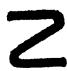
\includegraphics[keepaspectratio]{images/part002_56877e98.jpg}}

存在这样的拓扑除环，其中这一条件不满足，且其中环 \(\hat{\mathbf{K}}\) 有零因子（见习题 26）。此外，即使完备化 \(\hat{\mathbf{K}}\) 是拓扑除环，也没有先验的理由认为 \(\hat{\mathbf{K}}\) 的乘法一致结构是完备空间的结构。然而，对于除环 \(\mathbf{K}\)——只要 \(\hat{\mathbf{K}}\) 局部紧（见第一章，§ 9，第 7 节，命题 13，及第三章，§ 3，第 3 节，命题 4）——以及对于拓扑域，情形就是如此；对后者，我们有下列命题：

命题 8. 若拓扑域 K 的加法一致结构是完备豪斯多夫空间的结构，则 \(K^{*}\) 上的乘法一致结构是完备空间的结构。

我们将证明，若 \(\mathfrak{F}\) 是 \(\mathbf{K}^*\) 上关于乘法一致结构的 Cauchy 滤子，则 \(\mathfrak{F}\) 是 \(\mathbf{K}\) 上关于加法一致结构的 Cauchy 滤子，且不收敛于 \(o\)；这样就证得了结果。设 \(\mathbf{U}\) 是 \(o\) 在 \(\mathbf{K}\) 中的一个任意邻域，设 \(\mathbf{V}\) 是 \(o\) 的闭邻域，使得 \(\mathbf{V} \subset \mathbf{U}\)、\(\mathbf{VV} \subset \mathbf{U}\){[}公理 \((\mathrm{AV}_{\mathrm{II}})]\) 且 \(-1 \notin V\)；则按假设存在集合 \(\mathbf{A} \in \mathfrak{F}\)，使得对所有 \(x \in \mathbf{A}\) 与 \(y \in \mathbf{A}\)，有 \(x^{-1}y \in 1 + V\)。取 \(a \in \mathbf{A}\)，则 \(\mathbf{A} \subset a + aV\)，而 \(a + aV\) 是不含 \(o\) 的闭集；因此 \(o\) 不在 \(\mathbf{A}\) 的闭包中，从而不是 \(\mathfrak{F}\) 的聚点。设 \(\mathbf{W}\) 是 \(o\) 的邻域，使得 \(aW \subset V\){[}公理 \((\mathrm{AV}_{\mathrm{I}})]\)；则按假设存在集合 \(\mathbf{B} \in \mathfrak{F}\)，使得 \(\mathbf{B} \subset \mathbf{A}\)，且对所有 \(x \in B\) 与 \(y \in B\)，有 \(x^{-1}y \in 1 + W\)；于是 \(y - x \in xW \subset AW \subset aW + aVW\)；但 \(\mathbf{K}\) 交换，因此 \(aVW = aWV \subset VV \subset U\)；从而 \(y - x \in U + U\)，命题得证。

同样的证明表明，命题 8 可以推广到如下的情形：关于 K 的两个乘法一致结构之一的每个 Cauchy 滤子，也是关于另一个乘法一致结构的 Cauchy 滤子。

\section{拓扑群与拓扑环的逆极限}

在本节中，I 表示一个非空有向集（*），而 \(\alpha \leqslant \beta\) 表示 I 中的偏序关系。除非另有明确说明，所考虑的一切逆系统都以 I 为指标。
